\chapter{Preliminary Work}\label{C:preliminary}
This chapter presents the initial work conducted in investigating NSGA-II for the joint placement of container and VM. In this work, we consider the web services are deployed in containers, therefore, ``web service'' is used in the content instead of container. This work investigates the bilevel model including sub models (e.g power model), variables, and constraints. Two optimization objectives were initially considered: minimizing the energy consumption and the total price for the used VMs. A NSGA-II approach is applied for optimizing the problem. The result covers the evaluation of the proposed algorithm along with analysis, and concluding remarks and discussion of future work is given in conclusion (Section \ref{sec:con}). 
% \LaTeX\ is a very good tool for producing well-structured documents 
% carefully. It is very bad tool for banging things together in a rush 
% and panic. 

% \section{Floats}
% One perennial problem with \LaTeX\ is its treatment of 
% \emph{floats}.  Suppose you have a figure or table which you want to 
% include in your document. Where should it go? Traditional typesetting 
% practice is to put these in some convenient place, such as the top or 
% bottom of the current or next page, or at the end of the section or 
% chapter.  \LaTeX\ adopts a similar strategy, and allows floats to 
% ``float'' away from where they were defined. You can give a hint 
% about where you want the figure, but \LaTeX\ may move it. Sometimes 
% this is fine but sometimes you may want to have more control and 
% insist that a float goes \emph{here}. Anselm Lingau's 
% \textsf{float} package gives you this flexibility. For example, the following figure is an example of a non-floating float:

% \begin{fig}[H]
% \begin{center}
% \begin{tabular}{l|lll}
% $\delta$ & $\mathit{a}$ & $\mathit{b}$ & $\Lambda$ \\ \hline 
% $S_{1}$  & $\{\}$       & $\{\}$      & $\{S_{2}, S_{5}, S_{10}\}$\\
% $S_{2}$  & $\{S_{3}\}$  & $\{\}$      & $\{\}$\\
% $S_{3}$  & $\{S_{4}\}$  & $\{\}$      & $\{\}$\\
% $S_{4}$  & $\{S_{3}\}$  & $\{\}$      & $\{\}$\\
% $S_{5}$  & $\{\}$       & $\{S_{6}\}$ & $\{\}$\\
% $S_{6}$  & $\{\}$       & $\{S_{7}\}$ & $\{S_{8}\}$\\
% $S_{7}$  & $\{S_{6}\}$  & $\{\}$      & $\{\}$\\
% $S_{8}$  & $\{S_{9}\}$  & $\{\}$      & $\{\}$\\
% $S_{9}$  & $\{\}$       & $\{S_{8}\}$ & $\{\}$\\
% $S_{10}$ & $\{S_{11}\}$ & $\{\}$      & $\{\}$\\
% $S_{11}$ & $\{\}$       & $\{S_{10}\}$& $\{\}$\\ 
% \end{tabular}
% \caption{The transition function of an NFA with $\Lambda$  transitions}

% \end{center}
% \end{fig}

% On the other hand, Figure \ref{Fig:two} is a floating float. 



% \begin{fig}[tbh]
% \begin{center}
% \begin{tabular}{l|ll}
% $\delta''$ & $\mathit{a}$ & $\mathit{b}$ \\ \hline 
% $T_{1}$  & $T_{2}$ & $T_{3}$\\ 
% $T_{2}$  & $T_{4}$ & $T_{5}$\\ 
% $T_{3}$  & $T_{6}$ & $T_{7}$\\ 
% $T_{4}$  & $T_{8}$ & \\
% $T_{5}$  & $T_{10}$ & \\
% $T_{6}$  &  & $T_{11}$\\ 
% $T_{7}$  & $T_{3}$ & \\
% $T_{8}$  & $T_{4}$ & \\
% $T_{10}$  &  & $T_{5}$\\ 
% $T_{11}$  & $T_{6}$ & 
% \end{tabular}
% \caption{The transition function of an FA to accept 
% the same language.}
% \label{Fig:two}
% \end{center}
% \end{fig}

% You can define different types of new floats, and you can have tables 
% of them in the contents pages.


% \section{URL's}
% Use \verb=\url= from the \textsf{url} package to typeset URL's. Just 
% using \verb+\texttt+ or \verb+\tt+ does not work:

% \begin{itemize}
% \item \verb+\texttt{http://www.mcs.vuw.ac.nz/~neil/}+
% \item \verb+\url{http://www.mcs.vuw.ac.nz/~neil/}+
% \end{itemize}

% Give:
% \begin{itemize}
% \item \texttt{http://www.mcs.vuw.ac.nz/~neil/}
% \item \url{http://www.mcs.vuw.ac.nz/~neil/}
% \end{itemize}
% If you use the \textsf{hyperref} package then you can produce PDF 
% files with clickable hyperlinks using \verb=\url=.

% \section{Graphics and \LaTeX}
% \LaTeX\ offers rather poor support for the inclusion of graphics. 
% There are lots of ways to include pictorial material in \LaTeX, all 
% of which are deficient in some way or other. Look at \cite{GRM97GC} for a 
% description of them. If your document does need to have pictures in it 
% it is worth thinking about what is needed \emph{before} you generate 
% the pictures.

% \section{The bibliography}

% You should build up your bibliography as you go along.  Trying to get 
% the details of the bibliography correct at the end of the project is 
% hard work. Make sure that you record all the relevant details. Beware 
% that material on the internet is likely to change very rapidly. If you 
% are going to include material which is only available on the internet, 
% then you should probably include in the reference the date on which 
% you obtained the document.

% \section{Run \LaTeX, run}

% \LaTeX\ builds up information about your document for the table of 
% contents, references and so on at each run. This means that, for 
% example, the table 
% of contents is really the table of contents of the previous 
% compilation. You may need to run \LaTeX\ two or three times to let it 
% catch up with itself. If you have cross references within your 
% bibliography (for example two papers from the same collection, such 
% as \cite{Dum93a,Dum93b}) you may need to run 
% BibTeX more than once. 

% It is also possible that the table of contents file has garbage in 
% it, and will prevent the document from being compiled. This may 
% happen if you have had to abort compilation, due to a bug in the 
% source file. If this is the case then removing the \texttt{.toc} file 
% will usually solve the problem. You will have to fix the original 
% bug, of course.


% \section{Find out more by\ldots}
% You can find out more by:
% \begin{itemize}
% \item reading any one of a number of books, such as \cite{GMS94,Lam94}. The 
% VUW library has copies of these;
% \item visiting  the Comprehensive \TeX\ Archive Network (CTAN) at 
% \url{www.ctan.org};
% \item typing \texttt{latex} into Google.
% \end{itemize}

% It is \emph{highly unlikely} that you are the first person who ever 
% wanted to do what you want to do with \LaTeX. Therefore it is likely 
% that someone has already solved your problem: the real key to using  
% \LaTeX\ well is to make effective use of what other people have done.

% \section{Summary}
% In this chapter we explained some things about \LaTeX.



% Service Oriented Architecture (SOA) and Cloud computing have significantly reformed the software industry. SOA provides a decentralized application architecture which allows software composition and reuse in a large, global scale. Meanwhile, Cloud computing provides  a scalable, reliable, and flexible infrastructure to web services. 


% These advantages come from virtualization technology, which provides different level of isolation \cite{vm_technology}: workload-level and full virtualization. Container \cite{container} is one of the workload level virtualization which allows single-application workloads sharing operating system and physical resources such as CPU time and memory. Therefore, this technology improves the utilization of a single virtual machine. The full virtualization is used to partition physical machine into a number virtual machines (VMs) which enables VM migration. 

% As the dramatic increase of web services and cloud facilities, the management of resources has become a critical issue. 
% In recent years, as the power bill has become the largest fraction of the operating cost of Cloud facility \cite{Energy_6}, to reduce power consumption has become a paramount concern for Cloud service providers.
% In order to achieve that, a common approach is to re-allocate web services to a minimum number of physical machines (PMs) \cite{Energy_7}. 
% Therefore, idle computing servers are turned down or put into save mode. This optimization process, often called \textit{consolidation} involves with two levels of delivery mode, Software as a service (SaaS) and Infrastructure as a service (IaaS). Because of the complexity, consolidation tasks for IaaS and SaaS are often considered as separated tasks with different objectives. 
% For SaaS, the challenges concentrate on satisfying the Service Level Agreements (SLAs) with unpredictable requests using a minimum amount of resources. Whereas, for IaaS, the challenges are the VM migrations and 
% energy conservation.  

% There are extensive algorithms proposed for SaaS and IaaS levels of resource allocation \cite{Mazumdar20174, dubois2015autonomic}.
% Ref. \cite{Service_2} proposes a heuristic algorithm for service consolidation in a set of servers with minimizing costs while avoiding the overload of server and satisfying end-to-end response time constraints. 

% Ref. \cite{Energy_8} proposes two algorithms for energy efficient scheduling of VMs in Cloud, including an exact VM allocation algorithm which is an extended Bin-Packing approach, and a migration algorithm based on integer linear programming. 

% However, as the two levels of resource allocation are interact with each other, we believe they cannot be separated. They should be considered as one global optimization with multi-objectives from the perspectives of both service providers and cloud providers. Therefore, in this paper, we first propose a model for solving \textit{service resource allocation in Cloud (SRAC)}. Secondly, we propose a NSGA-II-based multi-objective algorithm with specifically designed operators to solve the problem. The two objectives are:

% \begin{enumerate}
%   \item propose a model for solving IaaS and SaaS resource allocation together
%   \item propose a NSGA-II-based algorithm to solve SRAC.
% \end{enumerate}


% The rest of the paper is organized as follows. Section \ref{sec:back} discusses the traditional 
% approaches for IaaS and SaaS and the power model for VM allocation. It will also introduce
% related works of evolutionary multi-objective optimization techniques. Section \ref{sec:problem} describes the 
% definition of the SRAC problem. Section \ref{sec:method} introduces the representation and genetic operators for SRAC problem. Section \ref{sec:exp} illustrates the experiment design, results and discussions. Section \ref{sec:con} draws a conclusion and discusses the future work.

% Copyright information



\section{Related models}
% Ref. \cite{ga_saas} proposes a single-objective genetic algorithm to solve placement of service (SaaS) on physical machines. Their major contributions are three-fold. Firstly, they consider web services as a workflow and optimize the makespan of a workflow. Secondly, they design a representation to the problem. Thirdly, they do not only consider computing 
% nodes, but storage nodes as well.
\subsection{Workload model}
Xavier el al \cite{Service_1} develops a \textit{Resource-Allocation-Throughput (RAT)} model for web service allocation. The \textit{RAT model} mainly defines several important variables for an atomic service which represents a software component. Based on this model, firstly, an atomic service's throughput equals its coming rate if the resources of the allocated VM are not exhausted. Secondly, increasing the coming rate will also increase an atomic service's throughput until the allocated resource is exhausted. Thirdly, when the resource is exhausted, the throughput will not increase as request increasing. At this time, the virtual machine reaches its capacity. 

% Beloglazov et al.  \cite{Energy_Service_2} propose two algorithms for VM allocation. The first one is a bin-packing algorithm, called Modified Best Fit decreasing (MBFD) which is used when a new VM allocation request arrives. The second algorithm, named Minimization of Migration, is used to adjust the current VMs’ allocation according to the CPU utilization of a physical machine. Their experiments have shown that these methods lead to a substantial reduction of energy consumption in Cloud data centers.

\subsection{Power Model}

Shekhar's research \cite{Energy_1} is one of the earliest in energy aware consolidation for cloud computing. They conduct experiments of independent applications running in physical machines. They explain that CPU utilization and disk utilization are the key factors affecting the energy consumption. They also find that only consolidating services into the minimum number of physical machines does not necessarily achieve energy saving, because the service performance degradation leads to a longer execution time, which increases the energy consumption. 

Bohra \cite{Energy_3} develops an energy model to profile the power of a VM. They monitor the sub-components of a VM which includes: CPU, cache, disk, and DRAM and propose a linear model (Eq~\ref{eq:vmeter}). 
Total power consumption is a linear combination of the power consumption of CPU, cache, DRAM and disk. The parameters
$\alpha$ and $\beta$ are determined based on the observations of machine running CPU and IO intensive jobs. 
\begin{equation}
\label{eq:vmeter}
  P_{(total)} = \alpha P_{\{CPU, cache\}} + \beta P_{\{DRAM, disk\}}
\end{equation}
Although this model can achieve an average of 93\% of accuracy, it is hard to be employed in solving SRAC problem, for the lack of data.

Beloglazov et al. \cite{Energy_Service_2} propose a comprehensive energy model for energy-aware resource allocation problem (Eq~\ref{eq:anton}). $P_{max}$ is the maximum power consumption when a virtual machine is fully utilized;
$k$ is the fraction of power consumed by the idle server (i.e. 70\%); and $u$ is the CPU utilization. This linear relationship between power consumption and CPU utilization is also observed by \cite{Energy_4, Energy_5}. 
\begin{equation}
\label{eq:anton}
  P(u) = k \cdot P_{max} + (1 - k) \cdot P_{max} \cdot u
\end{equation}


% \subsection{Multi-objective Evolutionary Optimization}
% A multi-objective optimization problem consists of multiple objective functions to be optimized.
% A multi-objective optimization problem can be stated as follows:
% \begin{align}
% \min \ \ & \vec{f}(\vec{x}) = (f_1(\vec{x}), \dots, f_m(\vec{x})), \\
% s.t. \ \ & \vec{x} \in \Omega.
% \end{align}
% where $\Omega$ stands for the feasible region of $\vec{x}$.

% Multi-objective Evolutionary Optimization Algorithm (MOEA) are ideal for solving multi-objective optimization problems \cite{MOEA}, because MOEAs work with a population of solutions. With an emphasis on moving towards the true Pareto-optimal region, a MOEA algorithm can be used to find multiple Pareto-optimal solutions in one single simulation run \cite{ope}. Therefore, this project would employ MOEA approaches. This is also the first time to employ MOEAs technique for SRAC problem.

\section{Problem Description}
\label{sec:problem}
We consider the problem as a multi-objective problem with two potentially conflicting objectives, 
minimizing the overall cost of web services and minimizing the overall energy consumption of the used physical machines. 

To solve the SRAC problem, we model an atomic service as its request and requests' coming rate, also known as frequency. 


The request of an atomic service is modeled as two critical resources: 
CPU time $A = \{A_1, A_i, \dots, A_t \}$ and 
memory consumption $M = \{M_1, M_i, \dots, M_t \}$, 
for each request consumes a $A_i$ amount of CPU time 
and $M_i$ amount of memory. 
The coming rate is denoted as $R = \{R_1, R_i, \dots, R_t \}$. 
In real world scenario, the size and the number of a request are both variant 
which are unpredictable, therefore, this is one of the major challenges in Cloud resource allocation. 
In this paper, we use fixed coming rate extracted from a real world dataset to represent real world service requests. 
 
The cloud data center has a number of available physical machines which are modeled as
CPU time $PA = \{PA_1, PA_j, \dots, PA_p\}$ and memory
$PM = \{PM_1, PM_j, \dots, PM_p\}$. $PA_j$ denotes the CPU capacity of a physical machine 
and $PM_j$ denotes the size of memory. A physical machine can be partitioned or
 virtualized into a set of virtual machines; 
 each virtual machine has its 
 CPU time $VA = \{VA_1, VA_n, \dots, VA_v\}$ and 
 memory $VM = \{VM_1, VM_n, \dots, VM_v\}$. 


The decision variable of service allocation is defined as $X^i_n$. $X^i_n$
is a binary value (e.g. 0 and 1) denoting whether a
service $i$ is allocated on a virtual machine $n$.
The decision variable of virtual machine allocation is defined as $Y^n_j$. $Y^n_j$
is also binary denoting whether a
VM $n$ is allocated on a physical machine $j$.


 In this work, we consider homogeneous physical machine which means physical machines have the same size of CPU time and memory. 
 The utilization of a CPU of a virtual machine is denoted as $U = \{U_1, U_n, \dots, U_v\}$. 
 The utilization can be calculated by Eq.\ref{eq:util}.

\begin{equation}
\label{eq:util}
  U_n =
  \begin{cases} 
    \frac{\sum_{i = 1}^t R_i \cdot A_i \cdot X^i_n}{VA_n}, \text{If }  \frac{\sum_{i = 1}^t R_i \cdot A_i \cdot X^i_n}{VA_n} < 1 \\
    1   \quad\quad\quad\quad\quad\quad\quad ,\text{otherwise}
  \end{cases}
\end{equation}

The cost of a type of virtual machine is denoted as $C = \{C_1, C_n \dots, C_v\}$. 



In order to satisfy the performance requirement, Service providers often define Service Level Agreements (SLAs) to ensure the service quality. In this work, we define throughput as a SLA measurement \cite{SLA_metric}. 
Throughput denotes the number of requests that a service could successfully process in a period of time. According to \textit{RAT} model, the throughput is equal to the number of requests when the allocated resource is sufficient. 
Therefore, if a VM reaches its utilization limitation, it means that the services have been allocated exceedingly.
Therefore, all services in that VM suffer from 
performance degradation.


Then we define two objective functions as the total energy consumption and the total cost of virtual machines:

\begin{equation}
\label{eq:energy}
\begin{aligned}
& {\text{minimize}}\\
& Energy = \sum\limits_{j=1}^p (k \cdot V_{max} + (1 - k) \cdot V_{max} \cdot \sum^v\limits_{n=1} U_n \cdot Y^n_j)\\
\end{aligned}
\end{equation}

\begin{equation}
\label{eq:cost}
\begin{aligned}
& & & & & & & Cost = \sum\limits_{j=1}^p\sum\limits_{n=1}^v C_n \cdot Y^n_j
\end{aligned}
\end{equation}

\subsubsection{Hard constraint}
A virtual machine can be allocated on a physical machine if and 
only if the physical machine has enough available capacity on every resource.

\begin{equation} 
\label{eq:constraint}
\begin{aligned}
\sum\limits_{n=1}^v VM_n \cdot Y^n_j \leq PM_j\\
\sum\limits_{n=1}^v VA_n \cdot Y^n_j \leq PA_j
\end{aligned}
\end{equation}

\subsubsection{Soft constraint}
A service can be allocated on a virtual machine even if the 
virtual machine does not have enough available capacity on every resource, but the allocated services will suffer from a quality 
degradation.
% For the soft constraint, we define that exceeding numbers of atomic services can still
%  be packed into a virtual machine, 
%  but if the resource of a virtual machine has been used up, all the applications 
%  in that VM will suffer from a quality degradation.
\begin{equation}
\sum\limits_{i=1}^t M_i \cdot R_i \cdot X_i^n  \leq VM_n
\end{equation}

\section{Methods}
\label{sec:method}
As we have discussed, Multi-objective Evolutionary Algorithms are good at solving 
multi-objective problems and NSGA-II \cite{nsgaii} has shown his effective and efficiency. NSGA-II is a well-known MOEA that has been widely used
in many real-world optimization problems. 
In this paper we also adopt NSGA-II to solve the SRAC problem. 
We first propose a representation and then present a NSGA-II based algorithm with novel genetic operators.

\subsection{Chromosome Representation}
SRAC is a two-level bin-packing problem, in the first level, 
bins represent physical machines and items represent virtual machines. Whereas, in the second level, a virtual machine acts like a bin and web services are items. 
Therefore, we design the representation in two hierarchies, virtual machine level and physical machine level. 

\begin{figure*}
\centering
  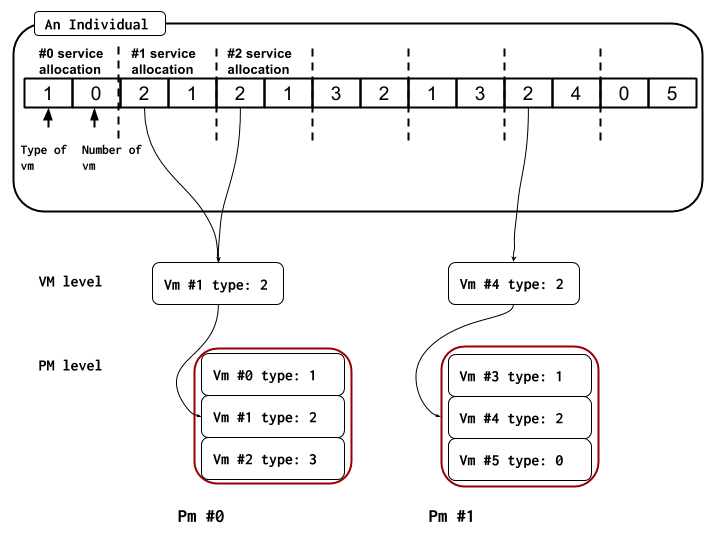
\includegraphics[width=0.8\textwidth]{pics/preliminary/cec.png}
  \caption{An example chromosome representation}
  \label{fig:rep}
\end{figure*}

Figure \ref{fig:rep} shows an example individual which contains seven service allocations. Each allocation of a service is represented as a pair where the index of each pair represents the number of web service. The first number indicates the type of virtual machine that the service is allocated in. The second number denotes the number of virtual machine.  For example, in Figure \ref{fig:rep}, service \#1 and service \#2 are both allocated in the virtual machine \#1 while service \#1 and service \#5 are allocated to different virtual machines sharing the same type.
The first hierarchy shows the virtual machine in which a service is allocated by defining VM type and number. 
Note that, the VM type and number are correlated once they are initialized. 
With this feature, the search procedure is narrowed down in the range of existing VMs which largely shrinks the search space.
The second hierarchy shows the relationship between a physical machine and its virtual machines, which are implicit. The physical machine is dynamically determined according to the virtual machines allocated on it. 
For example, in Figure ~\ref{fig:rep}, the virtual machines are 
sequentially packed into physical machines. The boundaries of PMs are calculated by adding up the resources of VMs until one of the resources researches the capacity of a PM. At the moment, no more VMs can be packed into the PM, then the boundary is determined.
% That is, we employ a simple heuristic method, 
% where the boundary of a physical machine is dynamically calculated. by adding up the virtual machines resources sequentially until a physical machine is full. 
The reason we designed this heuristic is because a physical machine is always fully used before launching another. Therefore, VM consolidation is inherently achieved.

Clearly, specifically designed operators are needed to manipulate chromosomes. Therefore, based on this representation, we further developed initialization, mutation, constraint handling and selection method.

\subsection{Initialization}
\begin{algorithm}[!htb]
 \caption{Initialization}
 \footnotesize
 \textbf{Inputs:} \\
  VM CPU Time $VA$ and memory $VM$, \\
  Service CPU Time $A$ and memory $M$ \\
  consolidation factor c \\
 \textbf{Outputs:}
  A population of allocation of services

 \begin{algorithmic}[1]
  \FOR{ Each service $t$ }
    \STATE{ Find its most suitable VM Type}
    \STATE{ Randomly generate a VM type $vmType$ which is equal
            or better than its most suitable type}
    \IF { There are existing VMs with $vmType$}
      \STATE randomly generate a number $u$
      \IF{ $u <$ consolidation factor }
      \STATE randomly choose one existing VM with $vmType$ to allocate
      \ELSE
      \STATE launch a new VM with $vmType$
      \ENDIF
    \ELSE
      \STATE Create a new VM with its most suitable VM type
    \ENDIF

  \ENDFOR
 \end{algorithmic}
 \label{alg:init}
\end{algorithm}


The initialization (see Alg~\ref{alg:init}) is designed to generate a diverse population.
In the first step, for each service, it is able to find the most suitable VM type which is just capable of running the service based on its resource requirements. 
In the second step, based on the suitable VM type, a stronger type is randomly generated. If there exists a VM with that type, the service is either deployed in the 
existing VM or launch a new VM. We design a consolidation factor $c$ which is a real number manually selected from 0 to 1 to control this selection. If a
random number $u$ is smaller than $c$, the service is consolidated in an existing VM.

This design could adjust the consolidation, therefore, controls the utilization of VM.

\subsection{Mutation}
\begin{figure}
\centering
  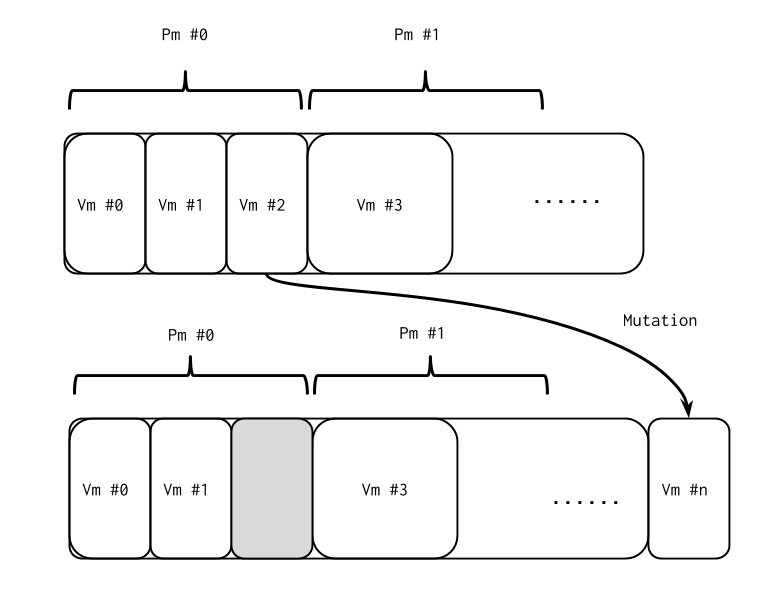
\includegraphics[width=0.7\textwidth]{pics/preliminary/hollow.png}
  \caption{An example mutation without insertion that causes a lower resource utilization}
  \label{fig:hollow}
\end{figure}

The design principle for mutation operator is to enable individuals exploring the entire feasible search space.
Therefore, a good mutation operator has two significant features, the exploration ability and the its ability to keep an individual within the feasible regions. In order to achieve these two goals, firstly, we generate a random virtual machine type which has a greater capacity than the service needs. It ensures the feasible of solutions as well as exploration capability. Then, we consider whether a service is consolidated with the consolidation factor $c$. 

The consolidation is conducted with a roulette wheel method which assigns fitness value to each VM according to the reciprocal of its current utilization. 
The higher the utilization, the lower the fitness value
it is assigned. 
Therefore, a lower utilization VM has a greater probability to be chosen. 
At last, if a new VM is launched, it will not be placed at the end of VM lists. Instead, it will be placed at a random position among the VMs. The reason is illustrated in Figure \ref{fig:hollow}. In the example, VM \#2 is mutated into a new type and be placed at the end of the VM list. However, because of the size of VM \#3 is too large for PM \#0, the hollow in PM \#0 will never be filled. This problem can be solved with the random insertion method.
\begin{algorithm}[!htb]
 \caption{Mutation}
 \footnotesize
 \textbf{Inputs:} \\
  An individual
  VM CPU Time $VA$ and memory $VM$, \\
  Service CPU Time $A$ and memory $M$ \\
  consolidation factor c \\
 \textbf{Outputs:}
  A mutated individual

 \begin{algorithmic}[1]
  \FOR{ Each service}
    \STATE Randomly generate a number $u$
    \IF { $u <$ mutation rate}
      \STATE find the most suitable VM Type for this service
      \STATE Randomly generate a number $k$
      \IF{ $k <$ consolidation factor }
        \STATE calculate the utilization of used VMs
        \STATE assign each VM with a fitness value of 1 / utilization and generate a roulette wheel
            according to their fitness values
        \STATE Randomly generate a number $p$, select the VM according to $p$
        \STATE Allocate the service
      \ELSE
        \STATE launch a new VM with the most suitable VM Type
        \STATE insert the new VM in a randomly choose position
      \ENDIF
    \ENDIF
  \ENDFOR
 \end{algorithmic}
 \label{alg:mutation}
\end{algorithm}

\subsection{Violation control method}
A modified violation ranking is proposed to deal with the soft constraint, for the hard constraint is automatically eliminated by the chromosome representation.
We define a violation number as the number of services which are allocated in the degraded VMs. 
That is, if there are excessive services allocated in a VM, then all the services are suffered from a degraded in performance. 
The violation number is used in the selection procedure, 
where the individuals with less violations are always preferred.

\subsection{Selection}
Our design uses the binary tournament selection with a constrained-domination principle. A constrained-domination principle is defined as following. A solution $I$ is considered constraint-dominate a solution $J$, if any of the following condition is true:
\begin{enumerate}
  \item Solution $I$ is feasible, solution is not,
  \item Both solutions are infeasible, $I$ has smaller overall
violations,
  \item Both solutions are feasible, solution $I$ dominates solution $J$.
\end{enumerate}

An individual with no or less violation is always selected. This method has been proved effective in the original NSGA-II paper \cite{nsgaii}.

\subsection{Fitness Function}
The cost fitness (Eq.\ref{eq:cost}) is determined by the type of VMs at which web service are allocated. 
The energy fitness is shown in Eq.\ref{eq:energy}, the utilizations (Eq.\ref{eq:util}) of VM are firstly converted into the utilizations of PM according to the proportion of VMs’ and PM’s CPU capacity.

\subsection{Algorithm}
The main difference between our approach and the original NSGA-II is that our approach has no crossover operator.

That is, a random switch of chromosome would completely destroy the order of VMs, 
hence, no useful information will be preserved. 
Therefore, we only apply mutation as the exploration method. Then, the algorithm becomes a parallel optimization without much interaction between its offspring, which is often addressed as Evolutionary Strategy \cite{evo_str}.
\begin{algorithm}[!htb]
 \caption{NSGA-II for SRAC}
 \footnotesize
 \textbf{Inputs:} \\
  VM CPU Time $VA$ and memory $VM$, \\
  PM CPU Time $PA$ and memory $PM$, \\
  Service CPU Time $A$ and memory $M$ \\
  consolidation factor c \\
 \textbf{Outputs:}
  A Non-dominated Set of solutions

 \begin{algorithmic}[1]
  \STATE Initialize a population $P$
  \WHILE{ Termination Condition is not meet}
    \FOR{ Each individual }
      \STATE Evaluate the fitness values
      \STATE Calculate the violation
    \ENDFOR

    \STATE non-Dominated Sorting of $P$
    \STATE calculate crowding distance
    \WHILE{ child number is less than population size }
      \STATE Selection
      \STATE Mutation
      \STATE add the child in a new population U
    \ENDWHILE
    \STATE Combine $P$ and $U$ \COMMENT{ for elitism}
    \STATE Evaluate the combined $P$ and $U$
    \STATE Non-dominated sorting and crowding distance for combined population
    \STATE Include the top popSize ranking individuals to the next generation

  \ENDWHILE
 \end{algorithmic}
 \label{alg:NSGAII}
\end{algorithm}

\section{Experiment}
\label{sec:exp}
\subsection{Dataset and Problem Design}
This project is based on both real-world datasets \textit{WS-Dream} \cite{Service_dataset} and simulated datasets \cite{Energy_9}. 
The \textit{WS-Dream} contains web service related datasets including network latency and service frequency (request coming rate). In this project, we mainly use the service frequency matrix. For the cost model, we only consider the rental of virtual machines with fixed fees (monthly rent). The configurations of VMs are shown in Table~\ref{tab:vm}, the CPU time and memory were selected manually and cost were selected proportional to their CPU capacity. The maximum PM's CPU and memory are set to 3000 and 8000 respectively. The energy consumption is set to 220W according to \cite{Energy_9}.

We designed six problems shown in Table \ref{tab:problem}, listed with increasing size and difficulty, which are used as representative samples of SRAC problem.

\begin{table}[]
\centering
\caption{Problem Settings}
\label{tab:problem}
\begin{tabular}{ccccccc}
\hline 

Problem           & 1  & 2  & 3  & 4  & 5   & 6    \\
Number of services & 20 & 40 & 60 & 80 & 100 & 200 \\ \hline
\end{tabular}
\end{table}

\begin{table}[]
\centering
\caption{VM configurations}
\label{tab:vm}
\begin{tabular}{@{}cccc@{}}
\toprule
VM Type & CPU Time & Memory & Cost \\ \midrule
1       & 250      & 500    & 25 \\
2       & 500      & 1000   & 50 \\
3       & 1500     & 2500   & 150\\
4       & 3000     & 4000   & 300\\ \bottomrule
\end{tabular}
\end{table}
\begin{flushleft}Selection Method with violation Control vs. without violation control\end{flushleft}
\begin{figure}
   \centering
   \begin{subfigure}[b]{0.45\textwidth} 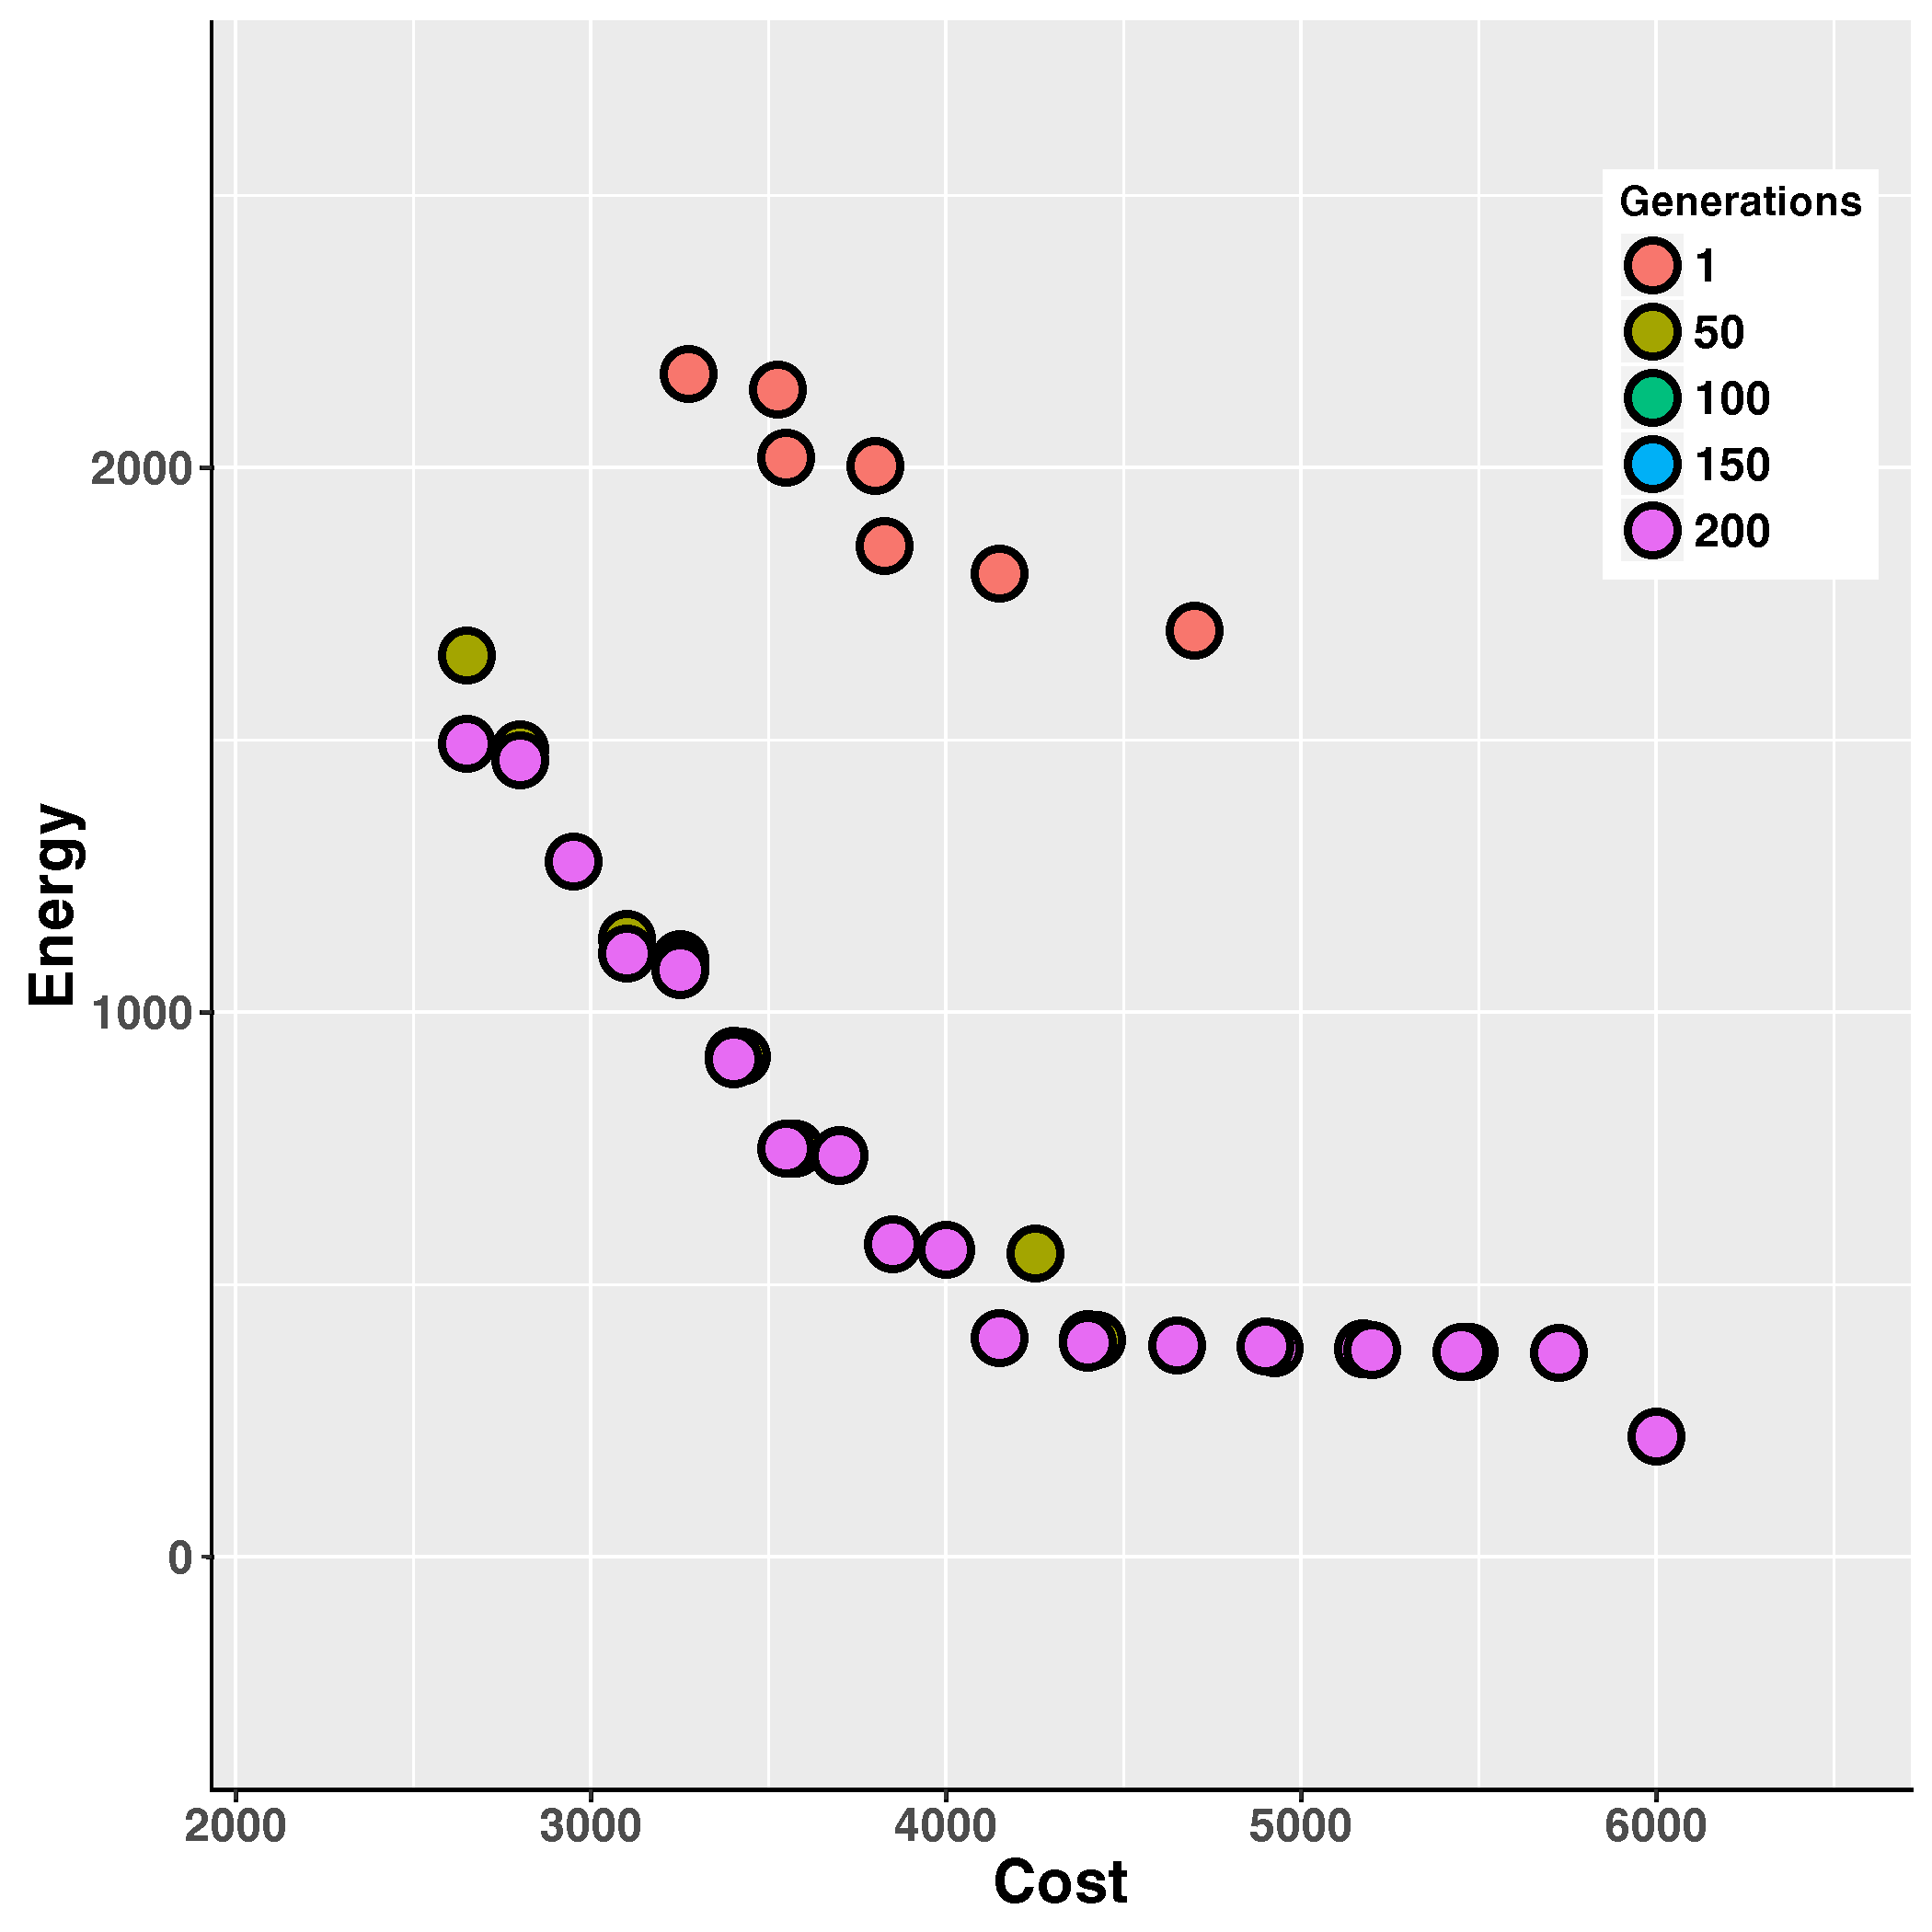
\includegraphics[width=\textwidth]{pics/preliminary/without/testCase1_.png}
   \caption{Problem 1}
   \label{fig:a}
   \end{subfigure}
   \begin{subfigure}[b]{0.45\textwidth} 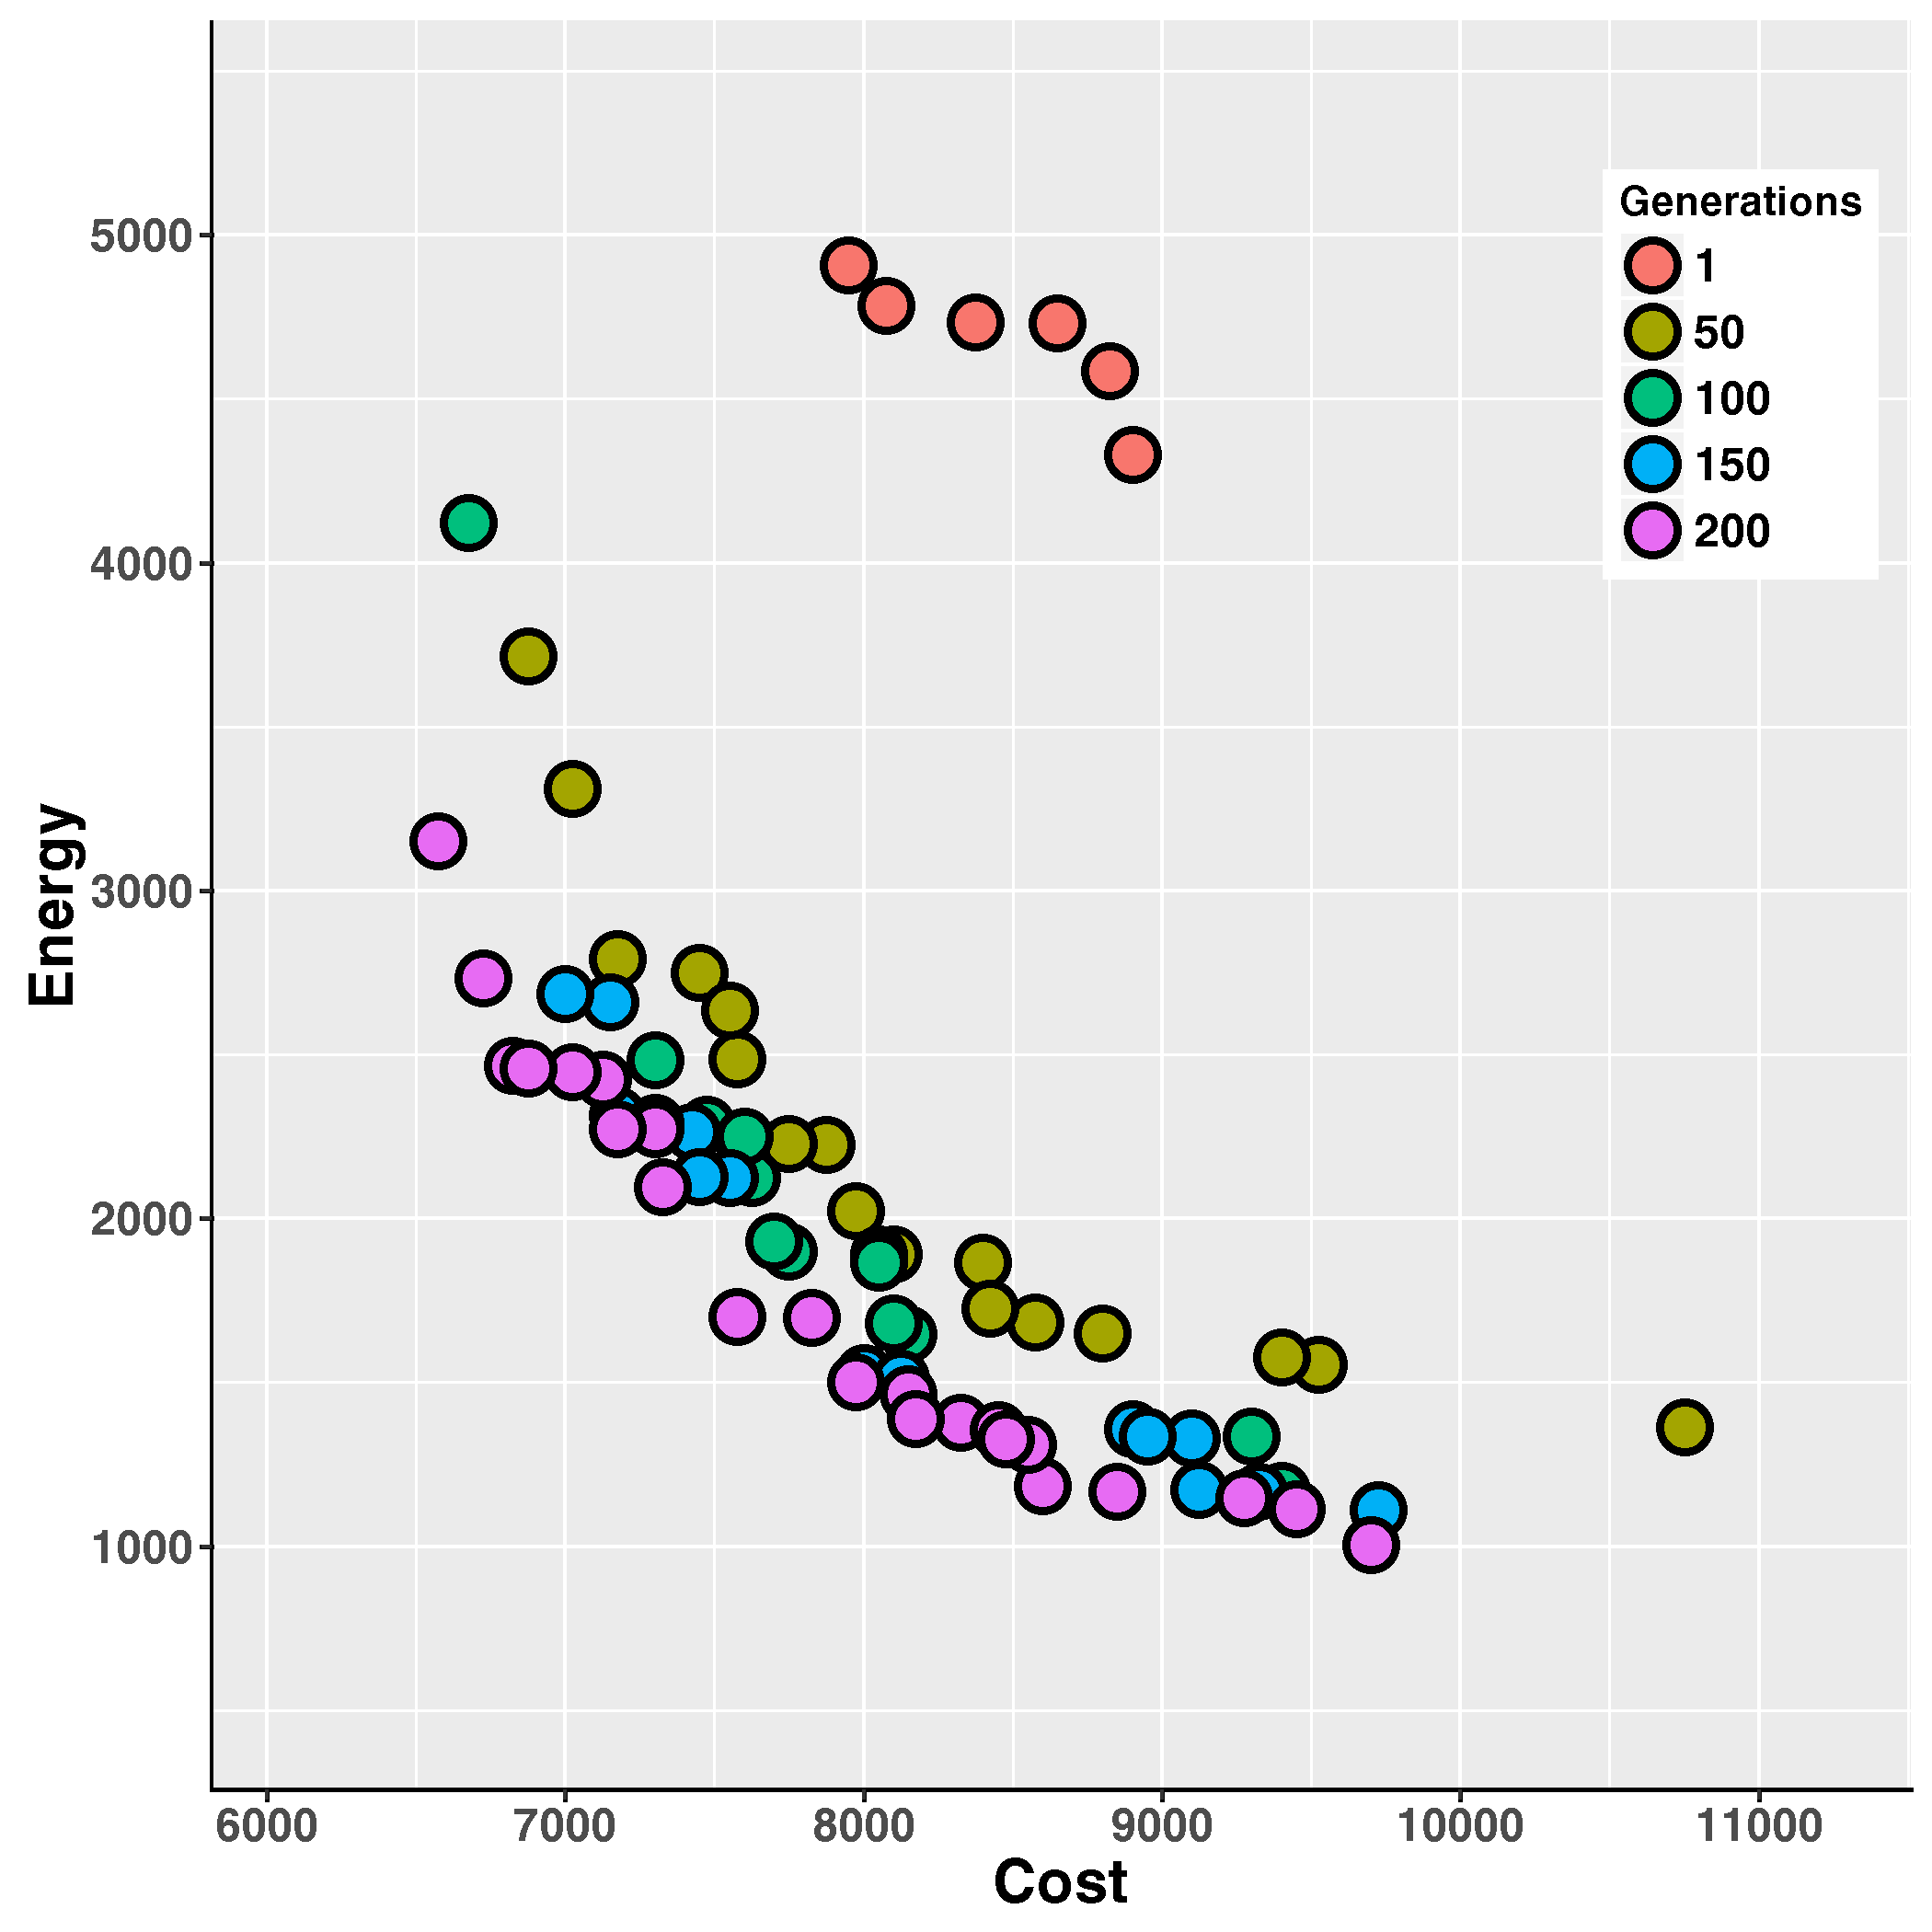
\includegraphics[width=\textwidth]{pics/preliminary/without/testCase2_.png}
   \caption{Problem 2}
   \label{fig:b}
   \end{subfigure}
   \begin{subfigure}[b]{0.45\textwidth}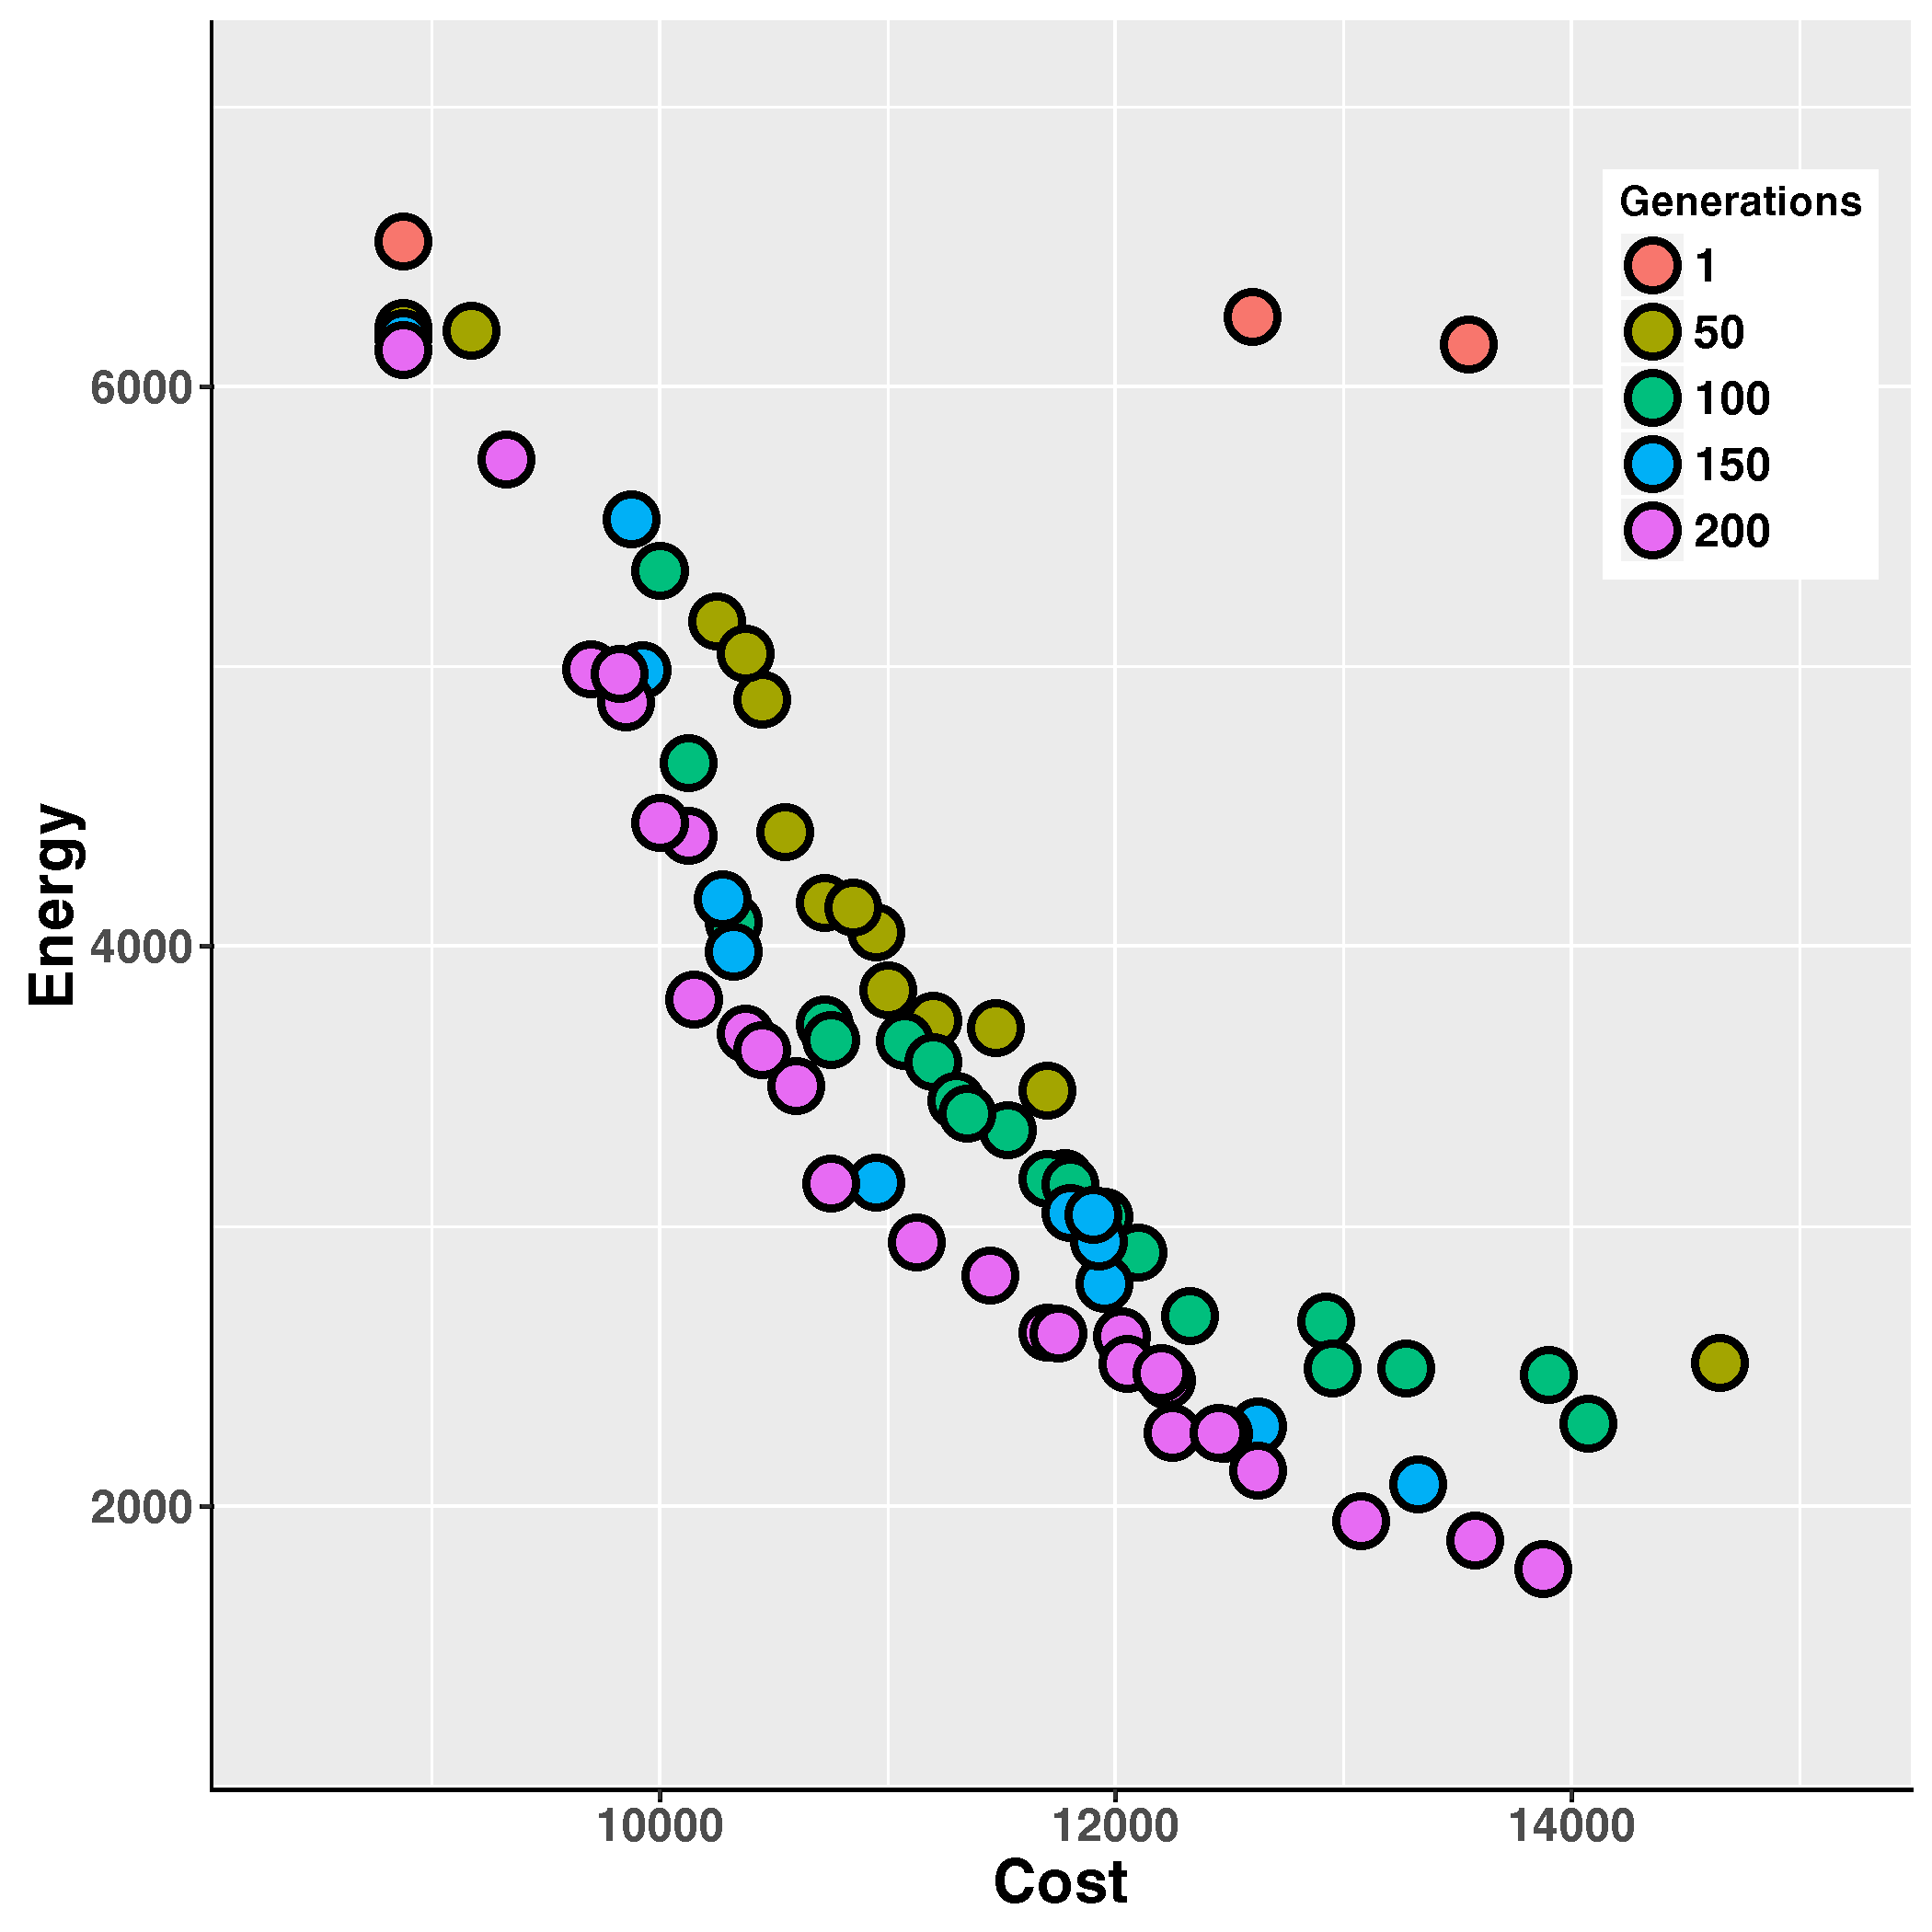
\includegraphics[width=\textwidth]{pics/preliminary/without/testCase3_.png}
   \caption{Problem 3}
   \label{fig:c}
   \end{subfigure}
   \begin{subfigure}[b]{0.45\textwidth}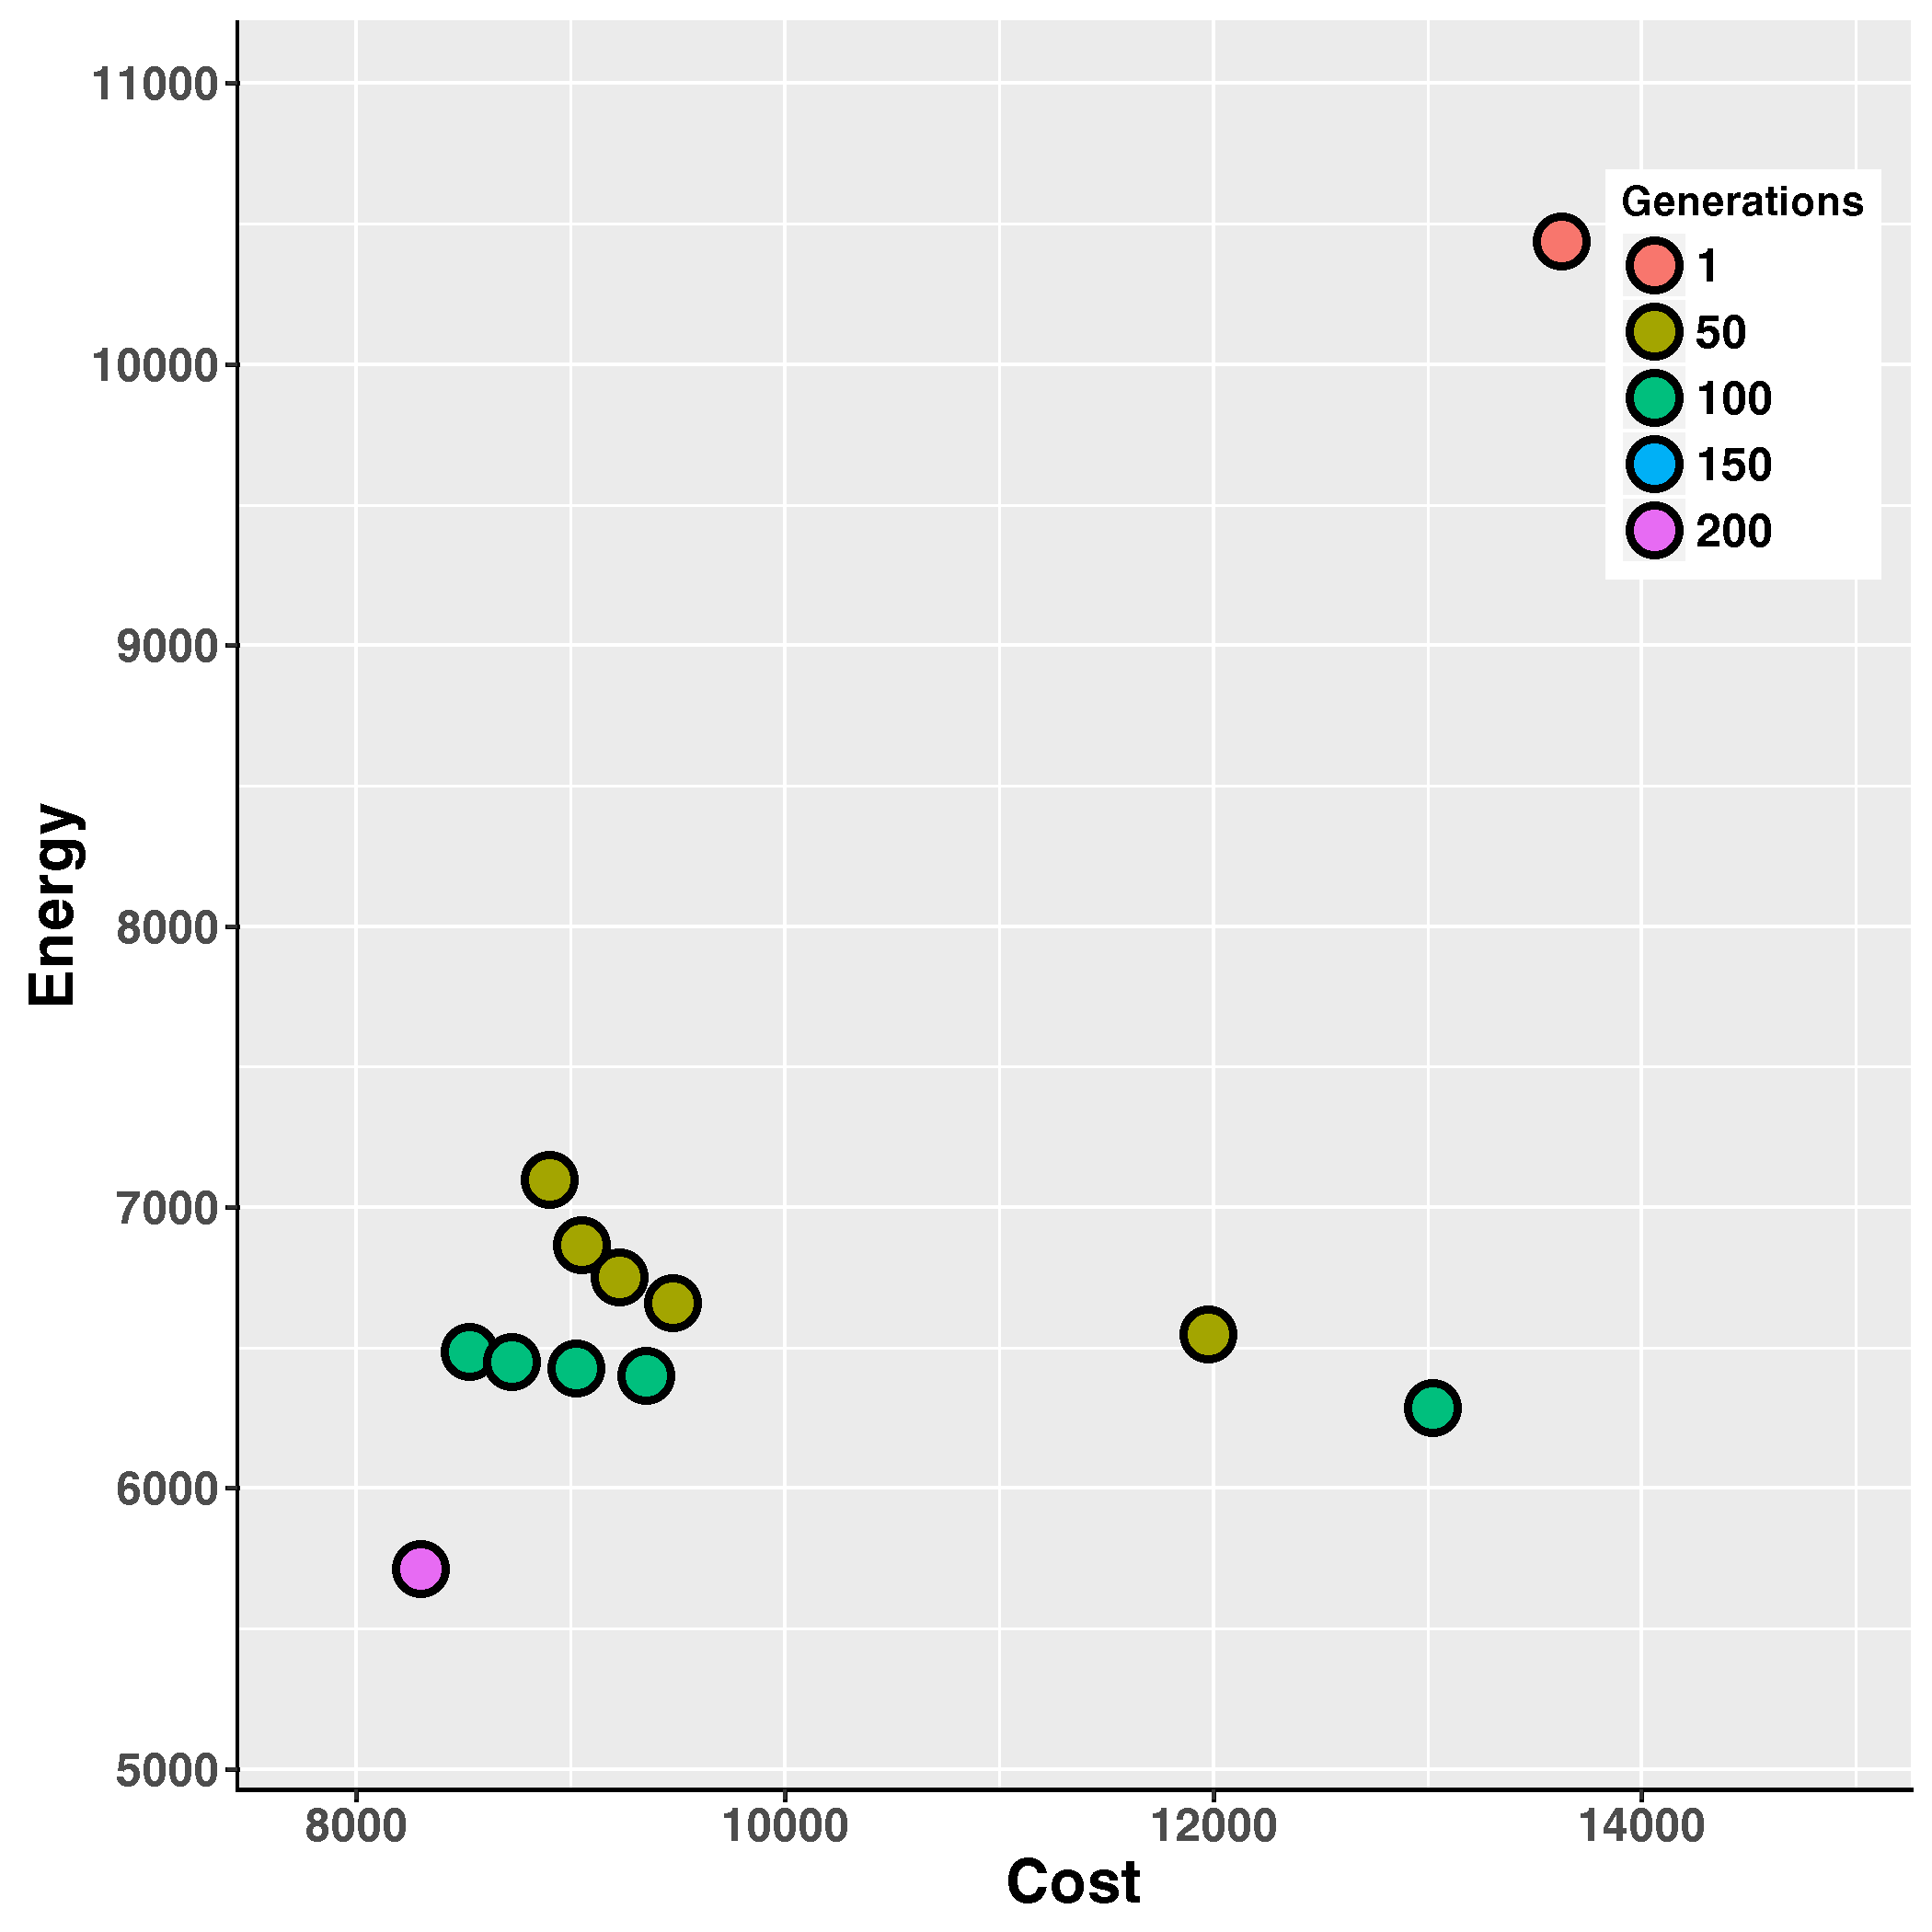
\includegraphics[width=\textwidth]{pics/preliminary/without/testCase4_.png}
   \caption{Problem 4}
   \label{fig:d}
   \end{subfigure}
   \begin{subfigure}[b]{0.45\textwidth}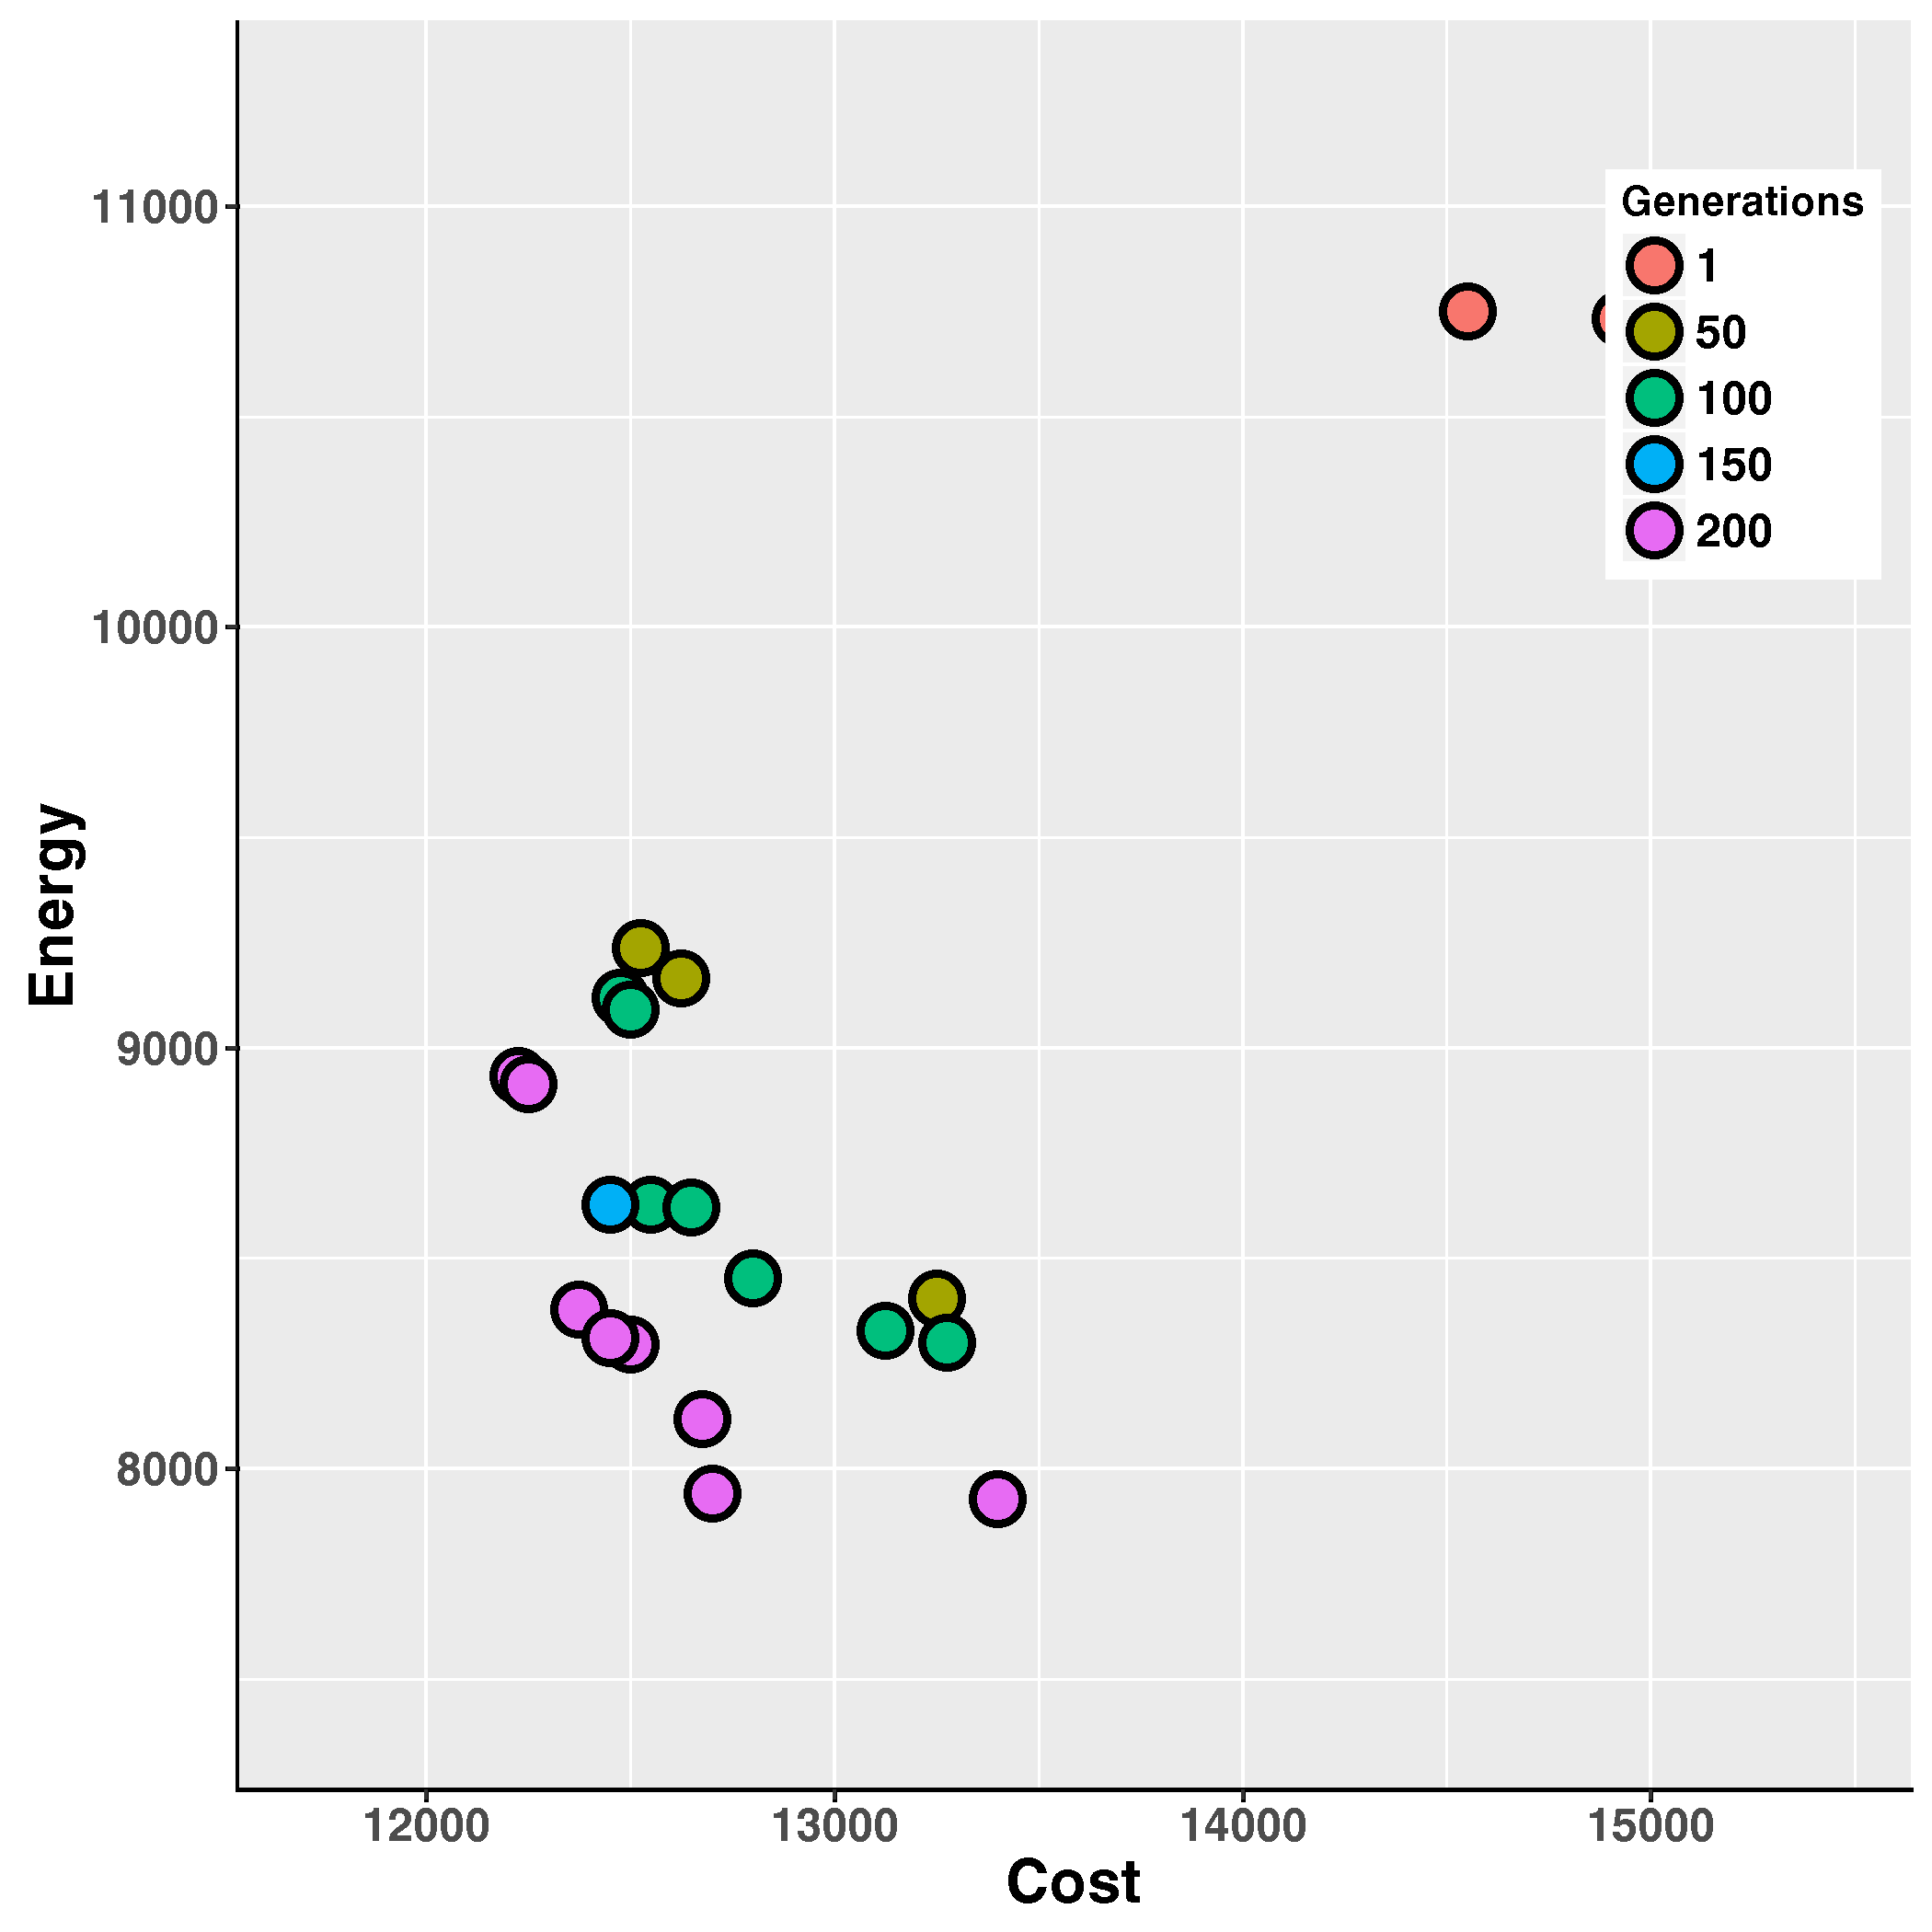
\includegraphics[width=\textwidth]{pics/preliminary/without/testCase5_.png}
   \caption{Problem 5}
   \label{fig:e}
   \end{subfigure}
   \begin{subfigure}[b]{0.45\textwidth}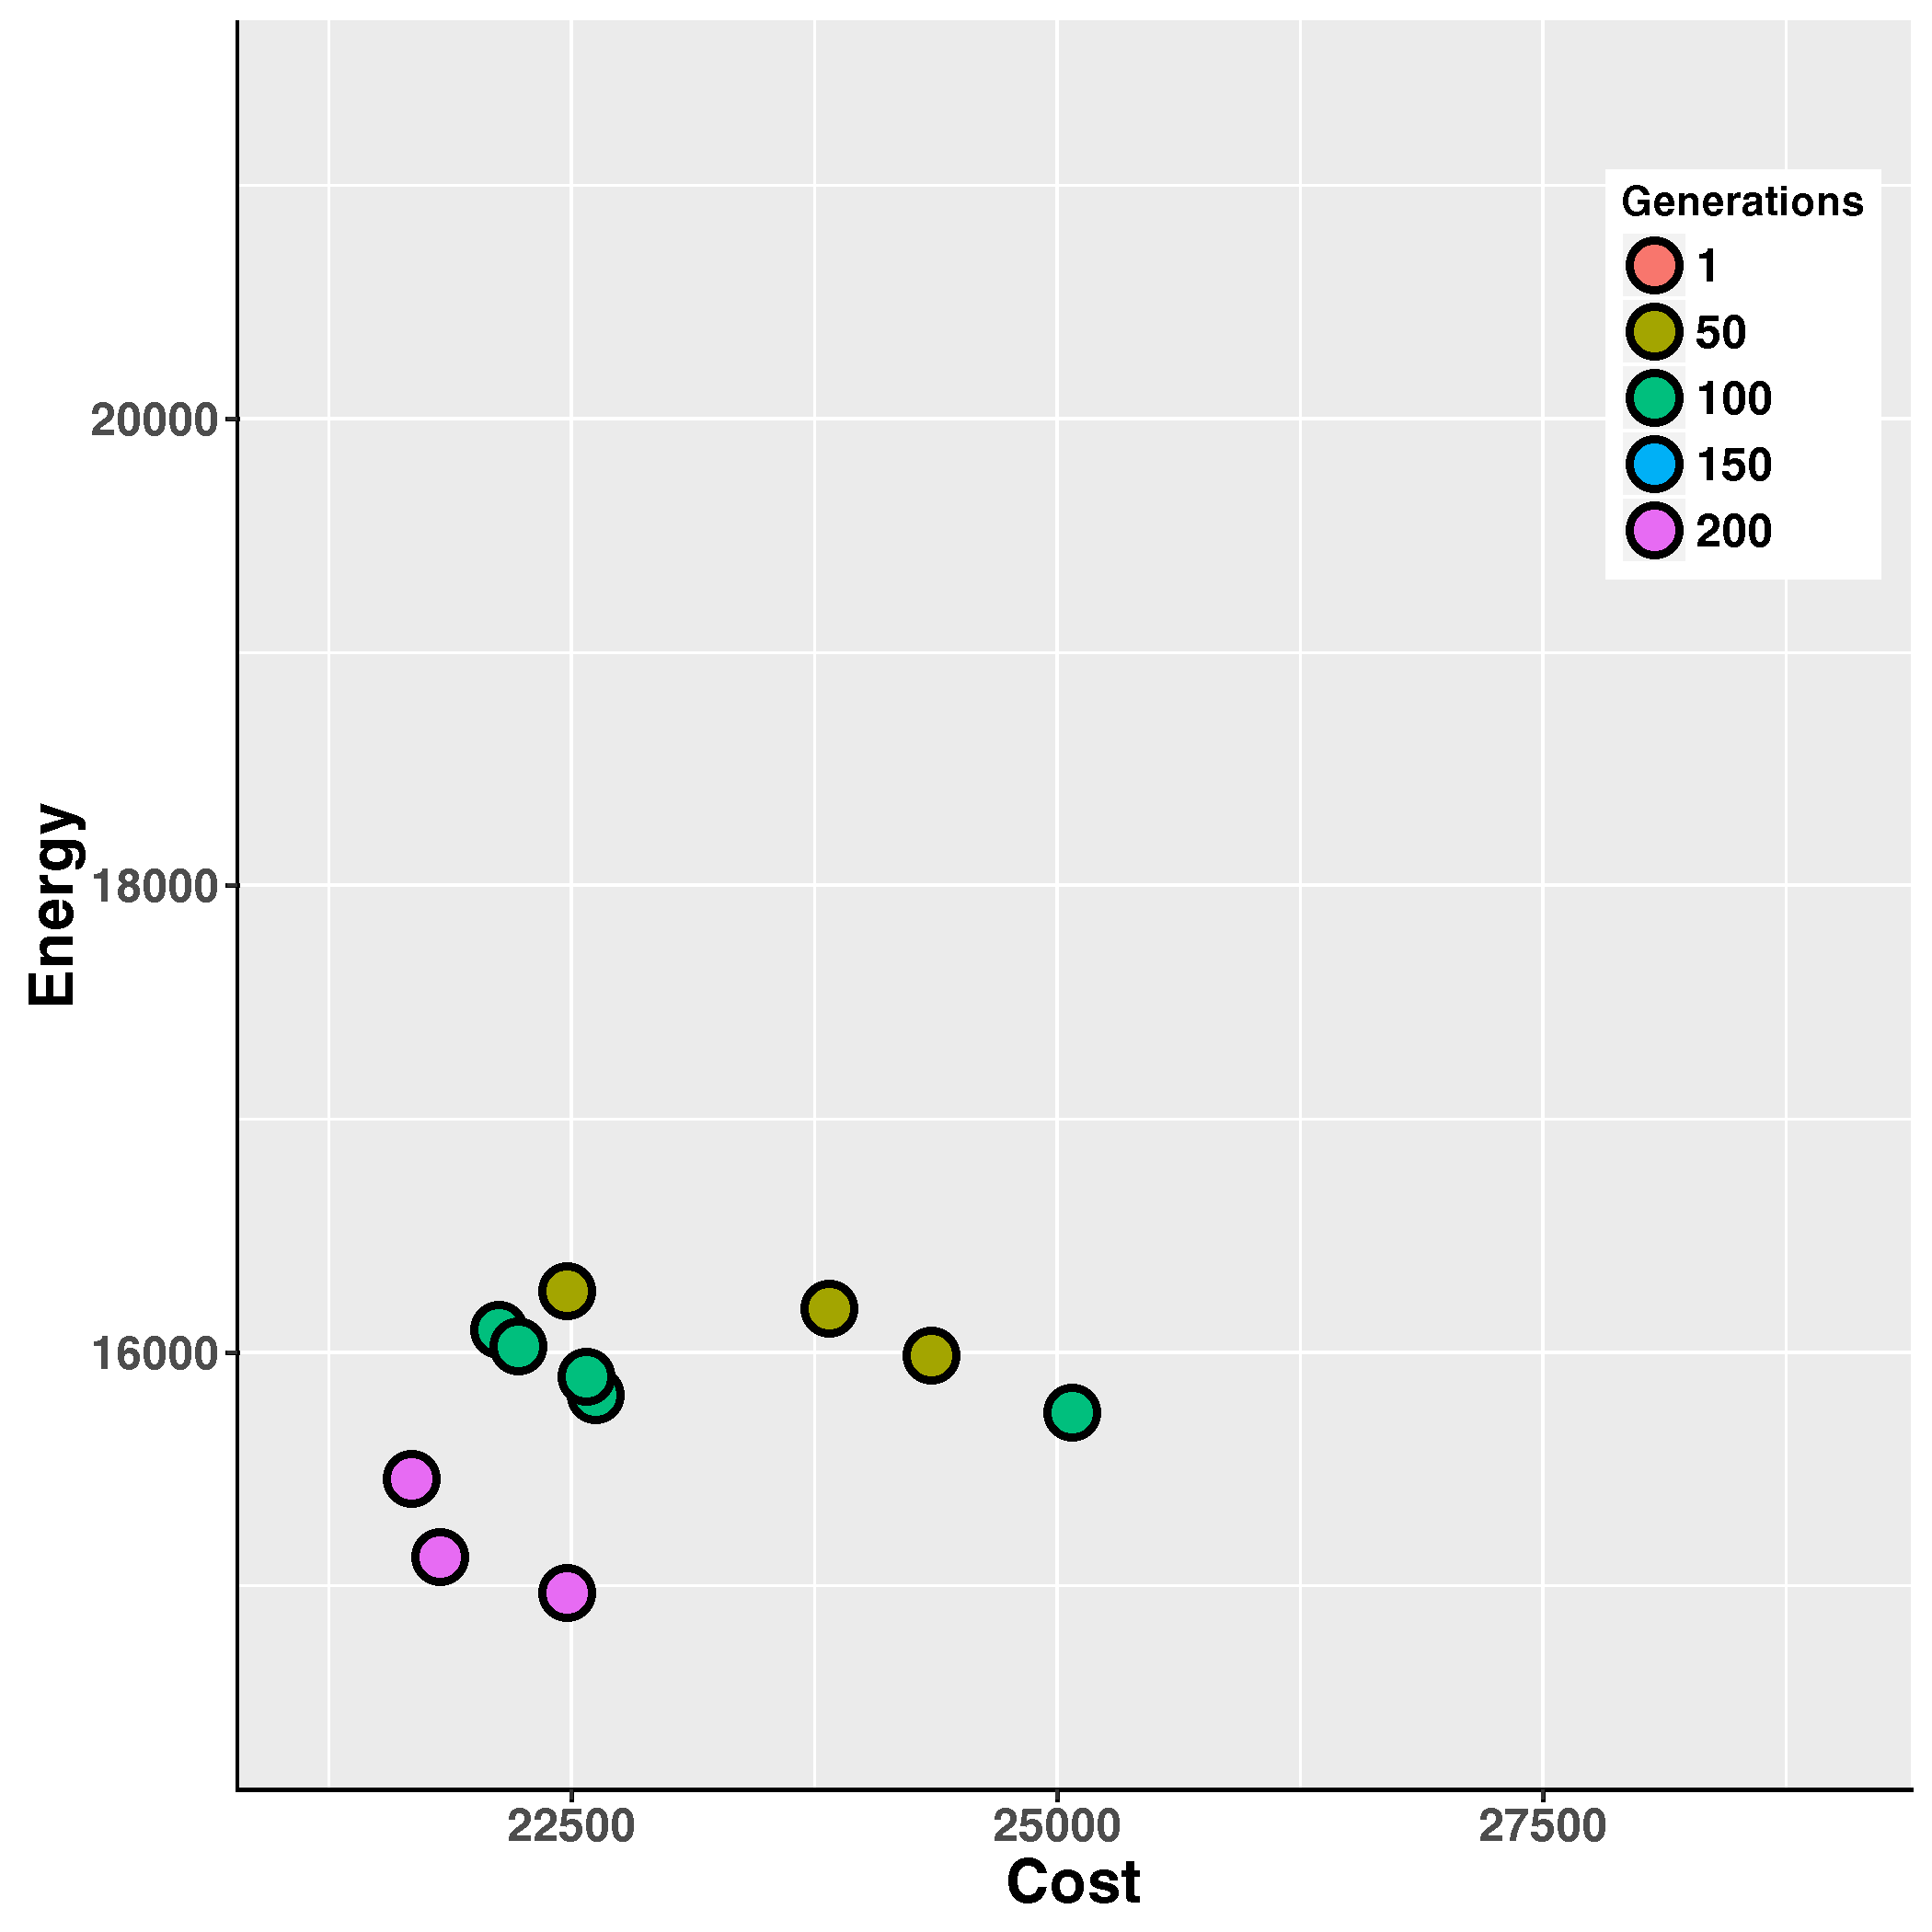
\includegraphics[width=\textwidth]{pics/preliminary/without/testCase6_.png}
   \caption{Problem 6}
   \label{fig:f}
   \end{subfigure}
   \caption{Non-dominated solutions evolve along with the generation}
   \label{fig:evolve}
\end{figure}

We conducted two comparison experiments. For the first experiment, we make a comparison between NSGA-II with violation control and NSGA-II without violation control. 
In second experiment, two mutation operators are compared. The first is the roulette wheel mutation, the second is the mutation with greedy algorithm. The mutation with greedy algorithm is a variant of roulette wheel mutation. The only difference is that instead of selecting a VM to consolidate with fitness values, it
always selects the VM with the lowest CPU utilization. 
Therefore, it is a greedy method embedded in the mutation.


The experiments were conducted on a personal laptop with 2.3GHz CPU and 8.0 GB
RAM. For each approach, 30 independent runs are performed for each problem with
constant population size 100. The maximum number of iteration is 200. $k$ equals 0.7. 
We set mutation rate and consolidation factor to 0.9 and 0.01.


\subsection{Results}
\begin{figure}
   \centering
   \begin{subfigure}[b]{0.45\textwidth}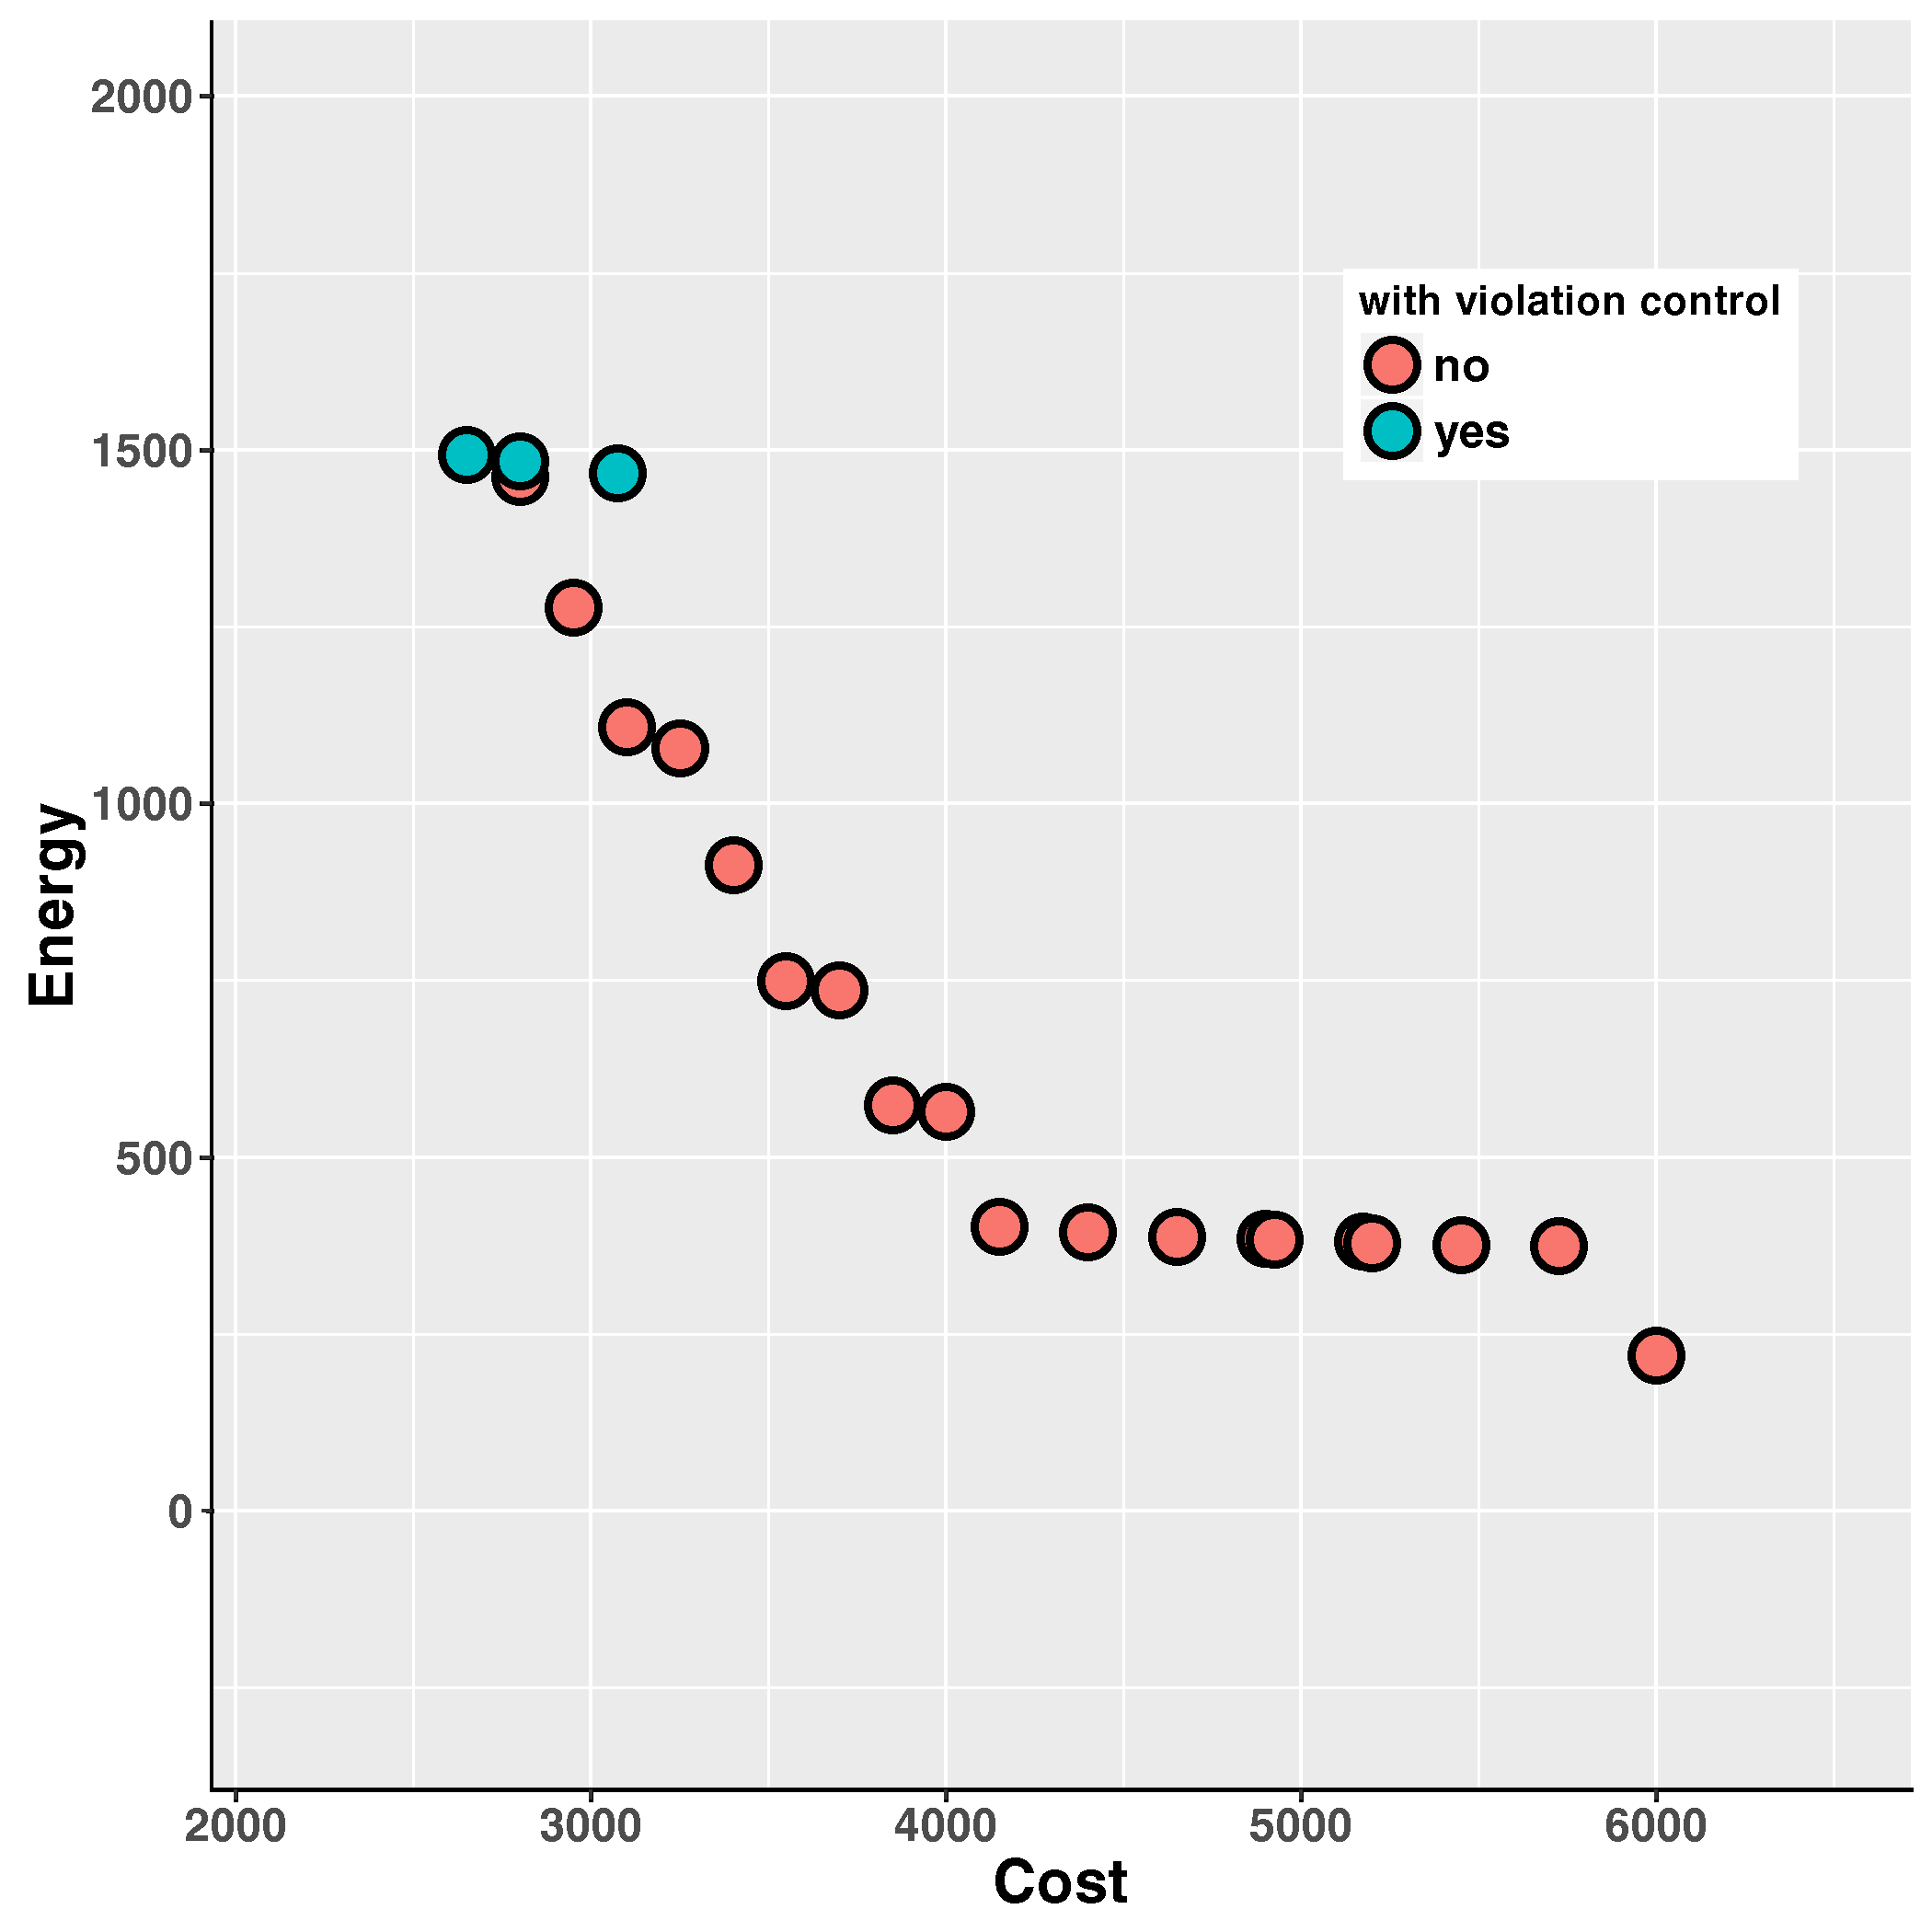
\includegraphics[width=\textwidth]{pics/preliminary/1/evolve.png}
   \caption{Problem 1}
   \label{fig:a}
   \end{subfigure}
   \begin{subfigure}[b]{0.45\textwidth}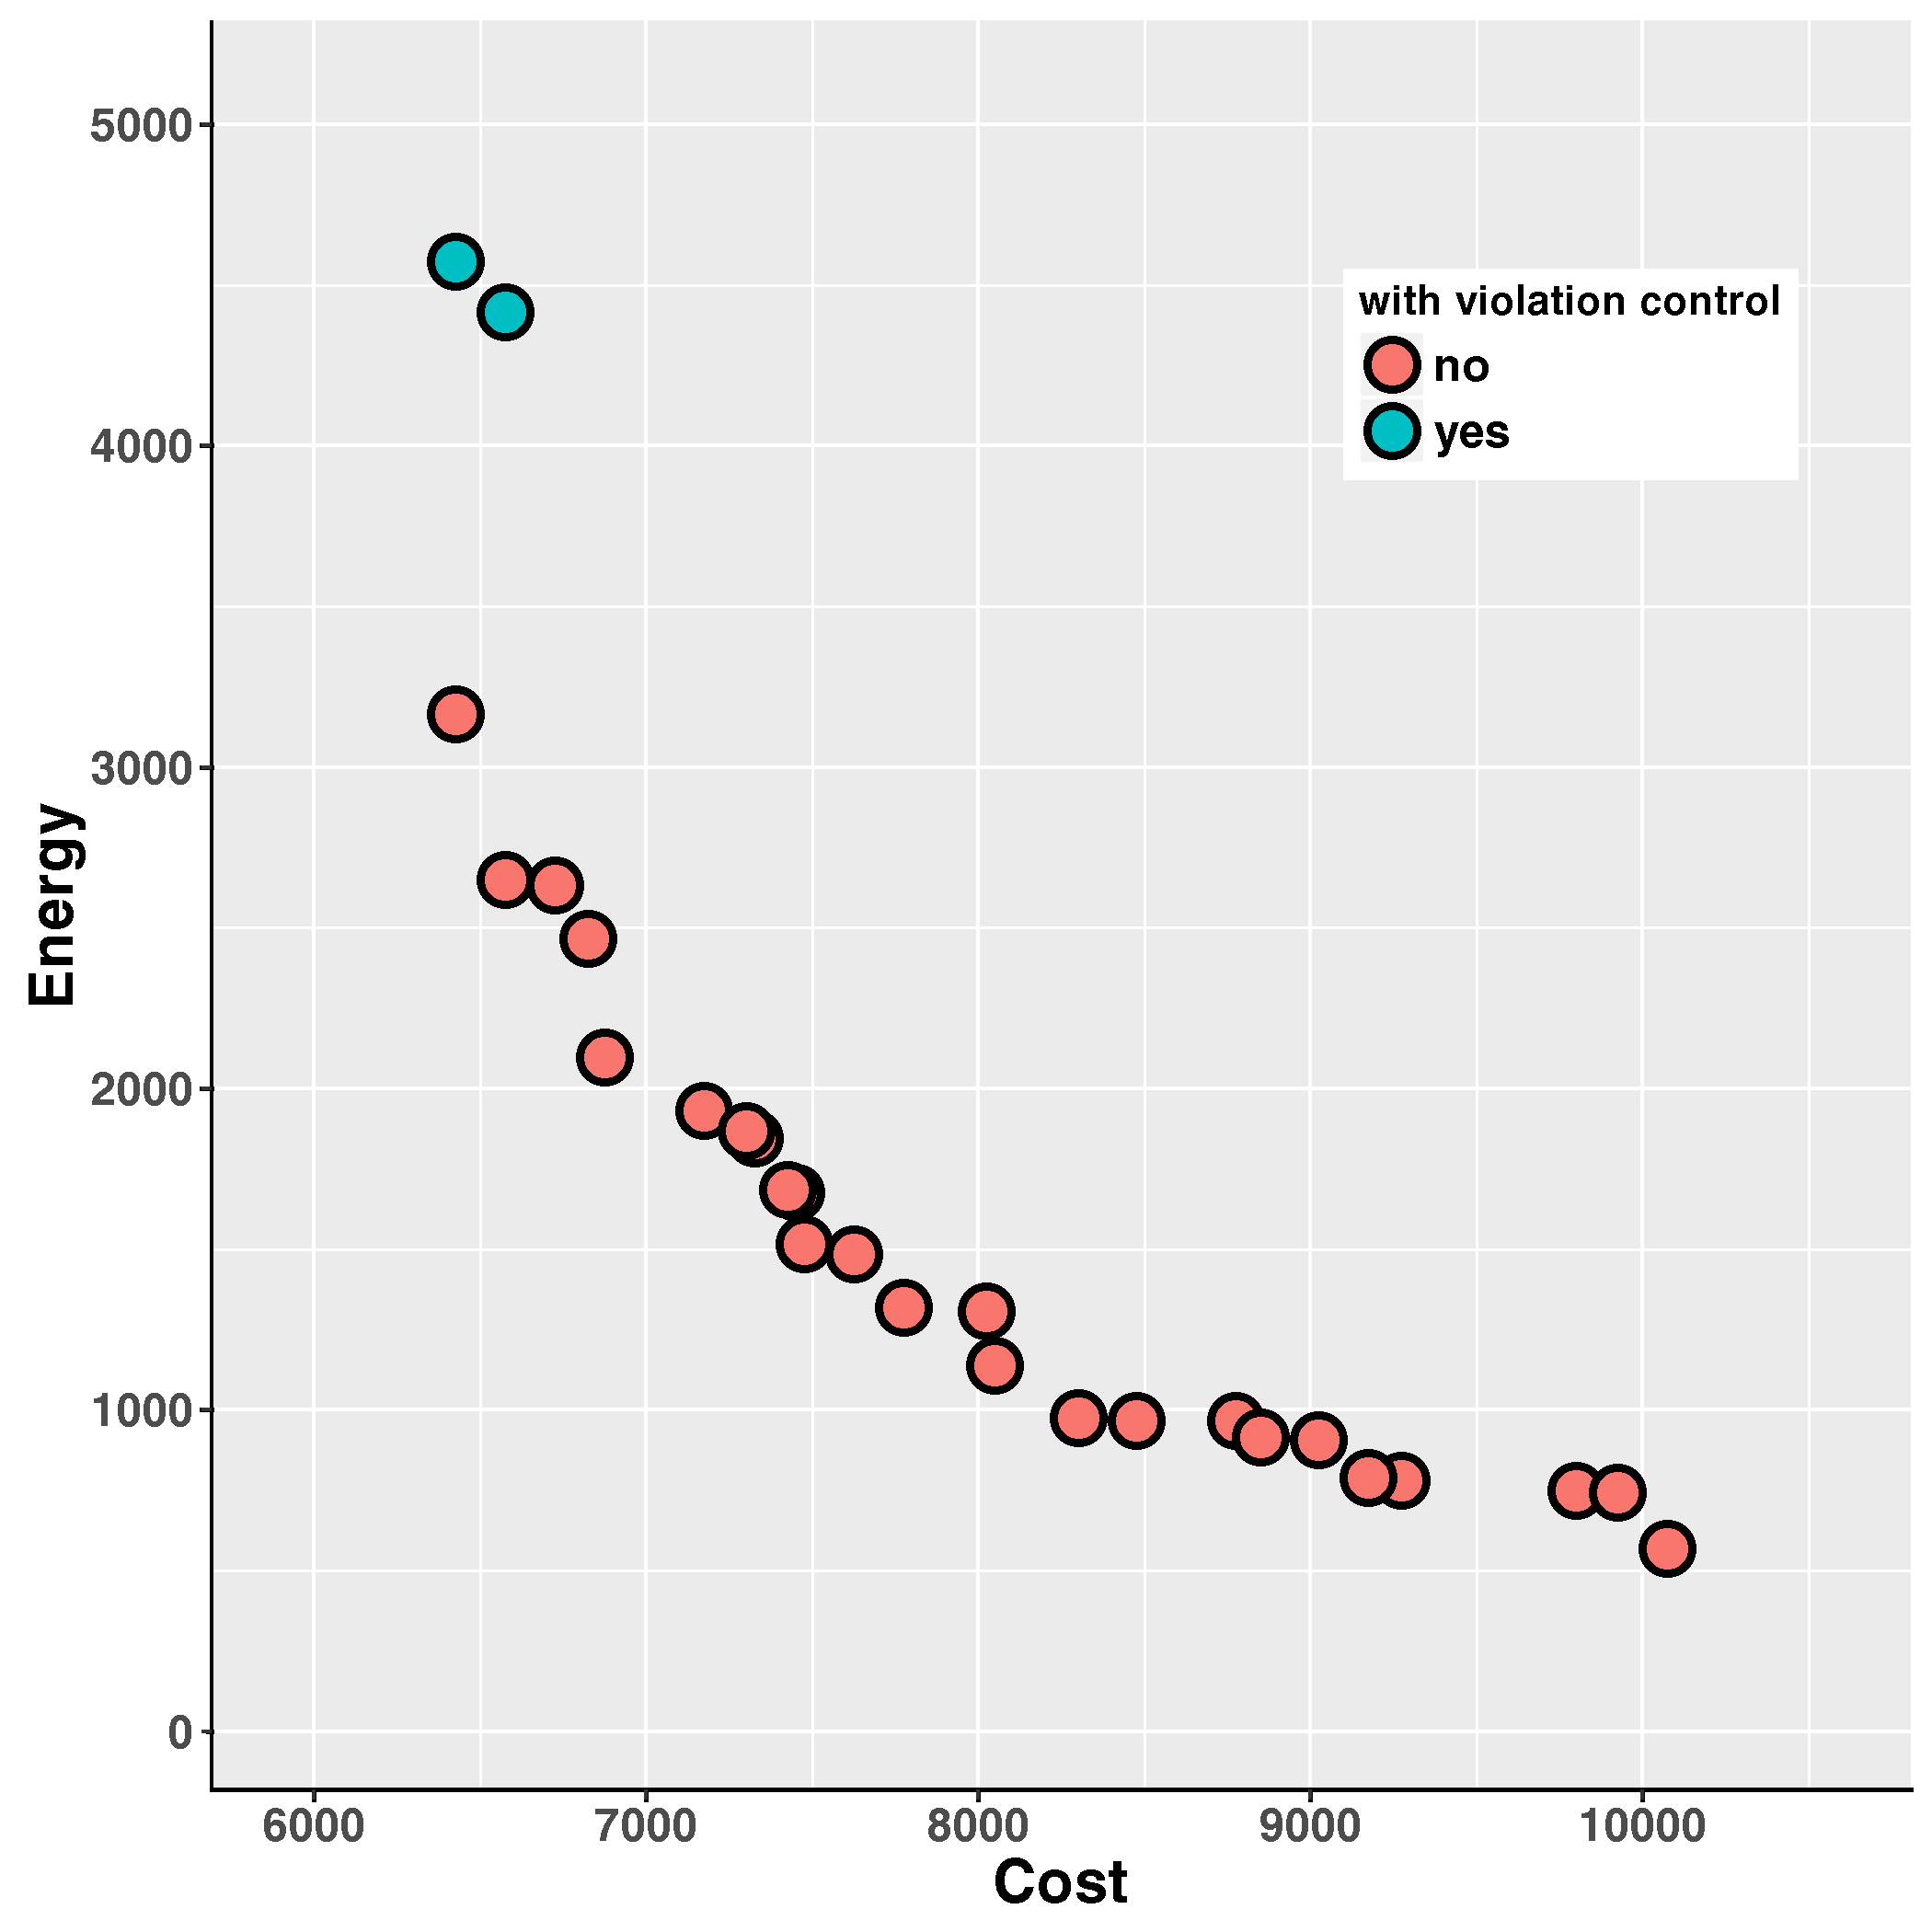
\includegraphics[width=\textwidth]{pics/preliminary/2/evolve.png}
   \caption{Problem 2}
   \label{fig:b}
   \end{subfigure}
   \begin{subfigure}[b]{0.45\textwidth}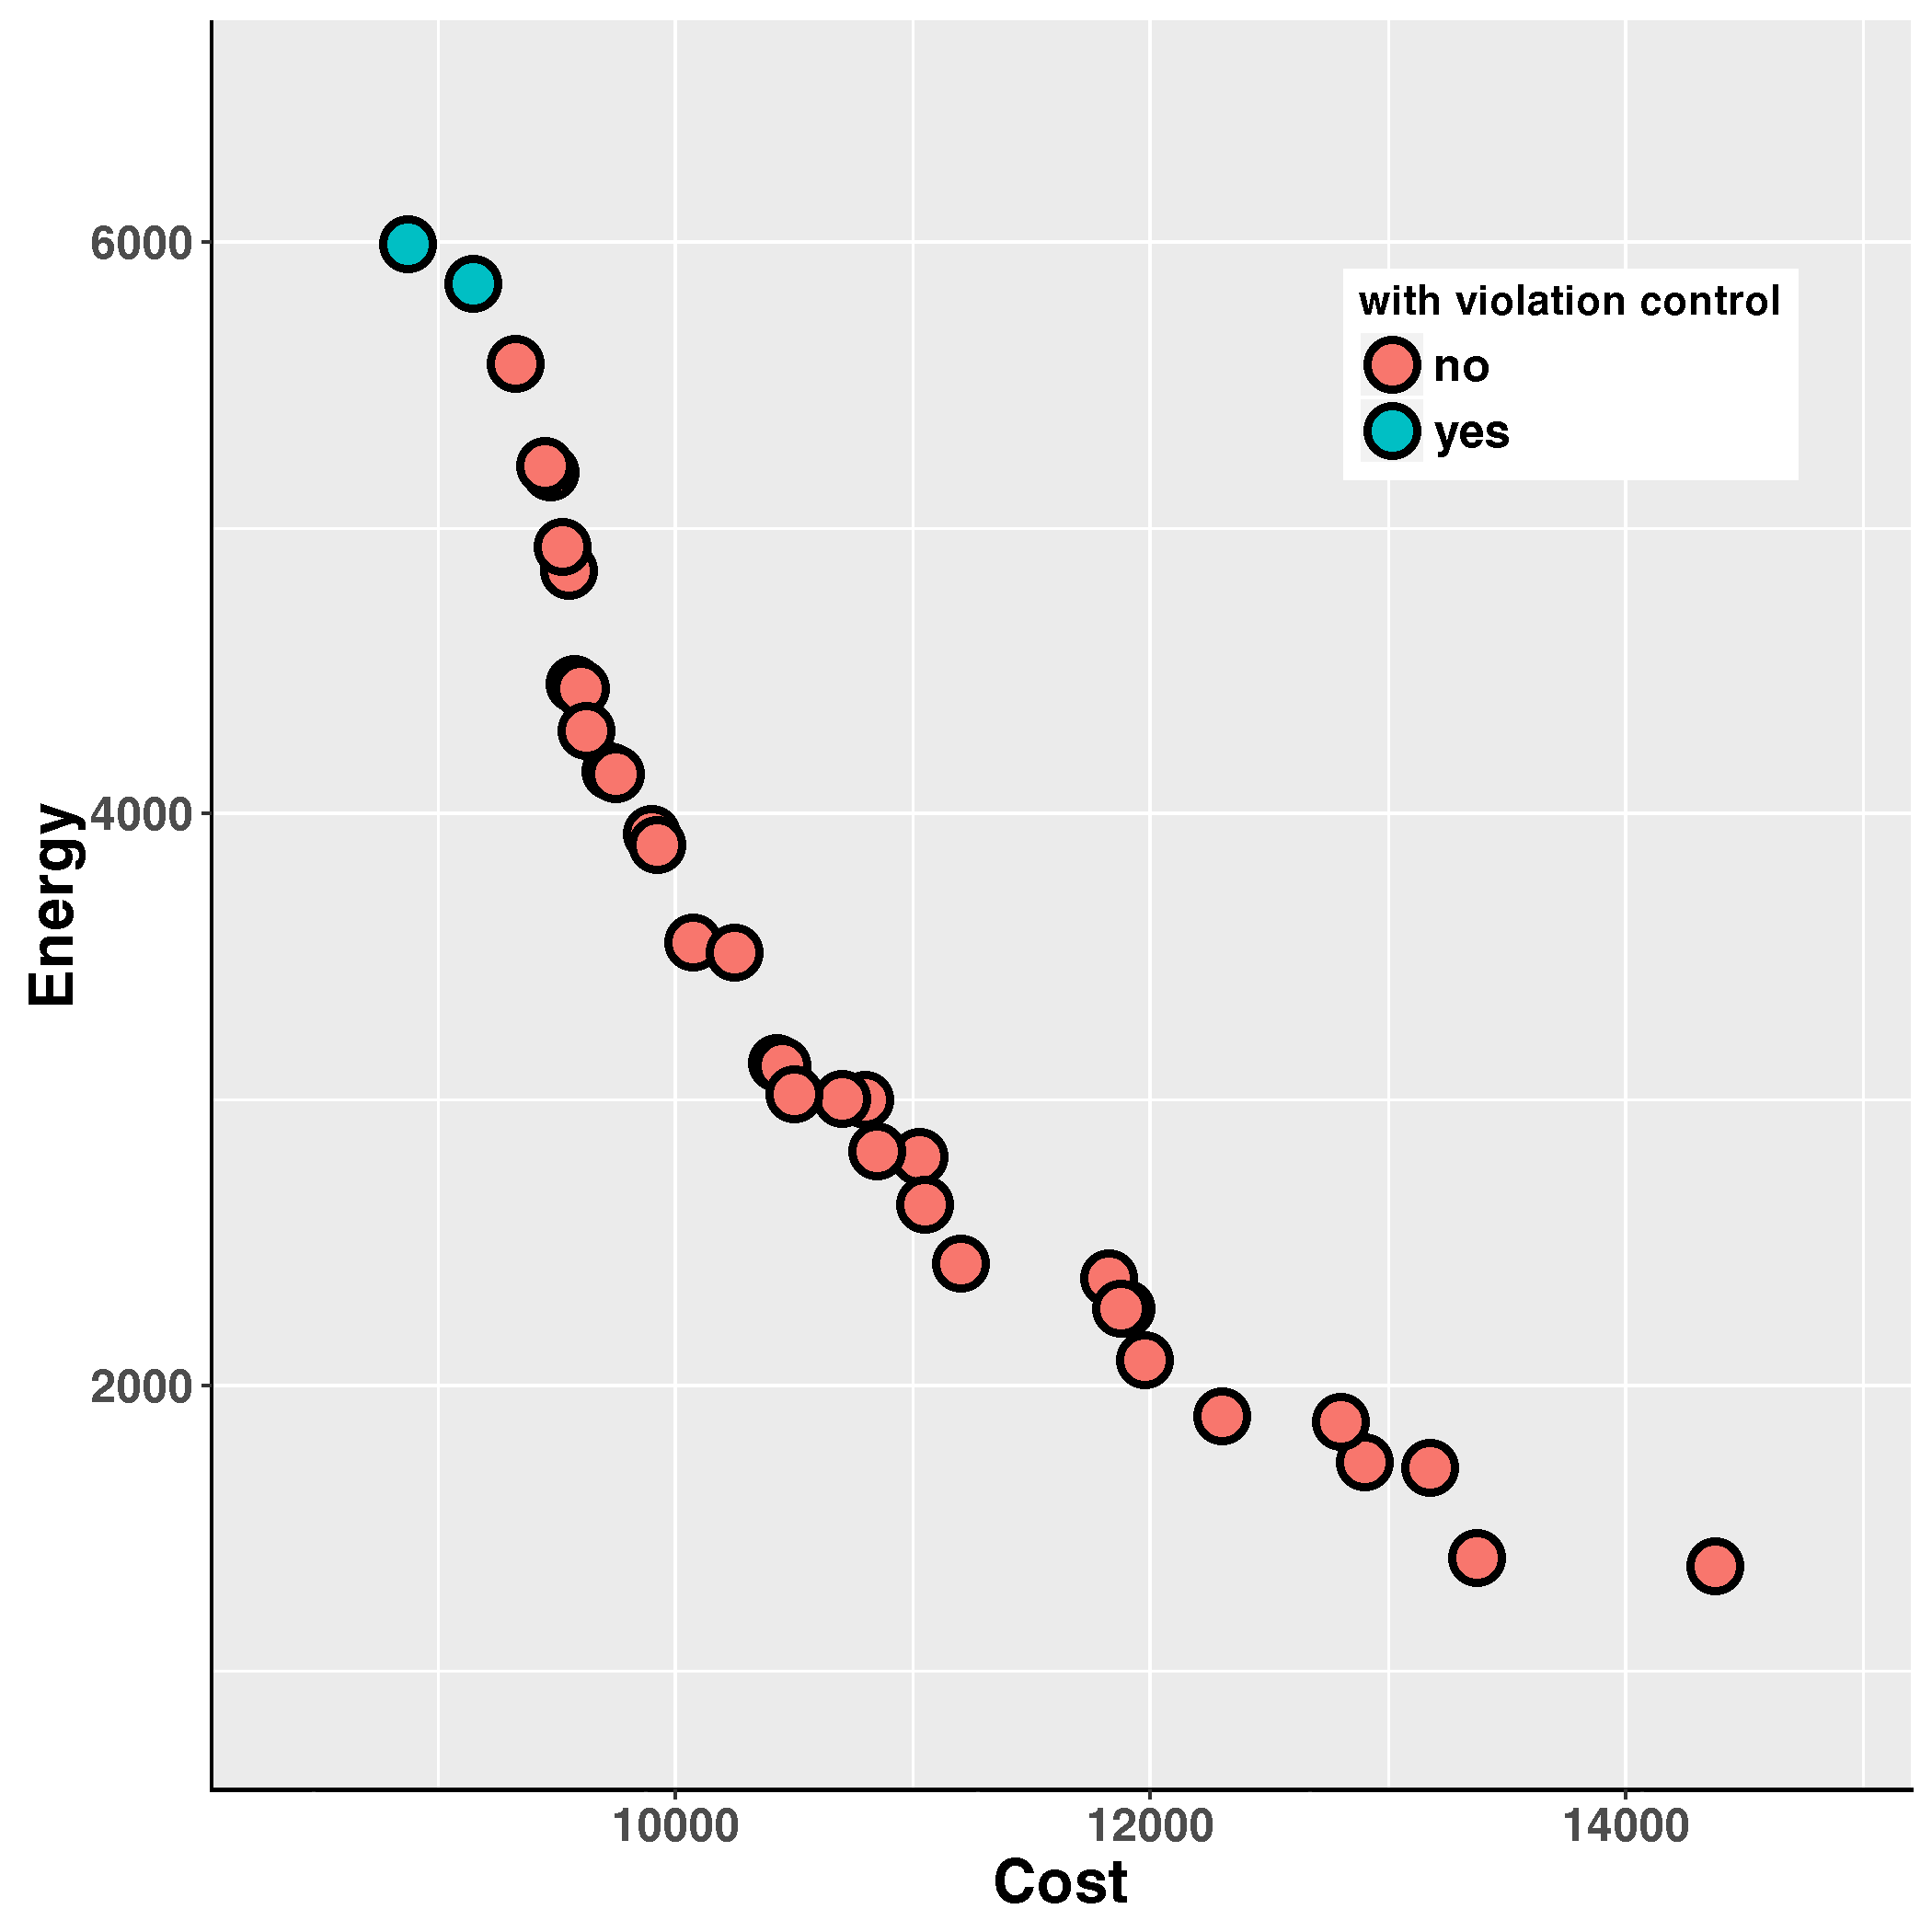
\includegraphics[width=\textwidth]{pics/preliminary/3/evolve.png}
   \caption{Problem 3}
   \label{fig:c}
   \end{subfigure}
   \begin{subfigure}[b]{0.45\textwidth}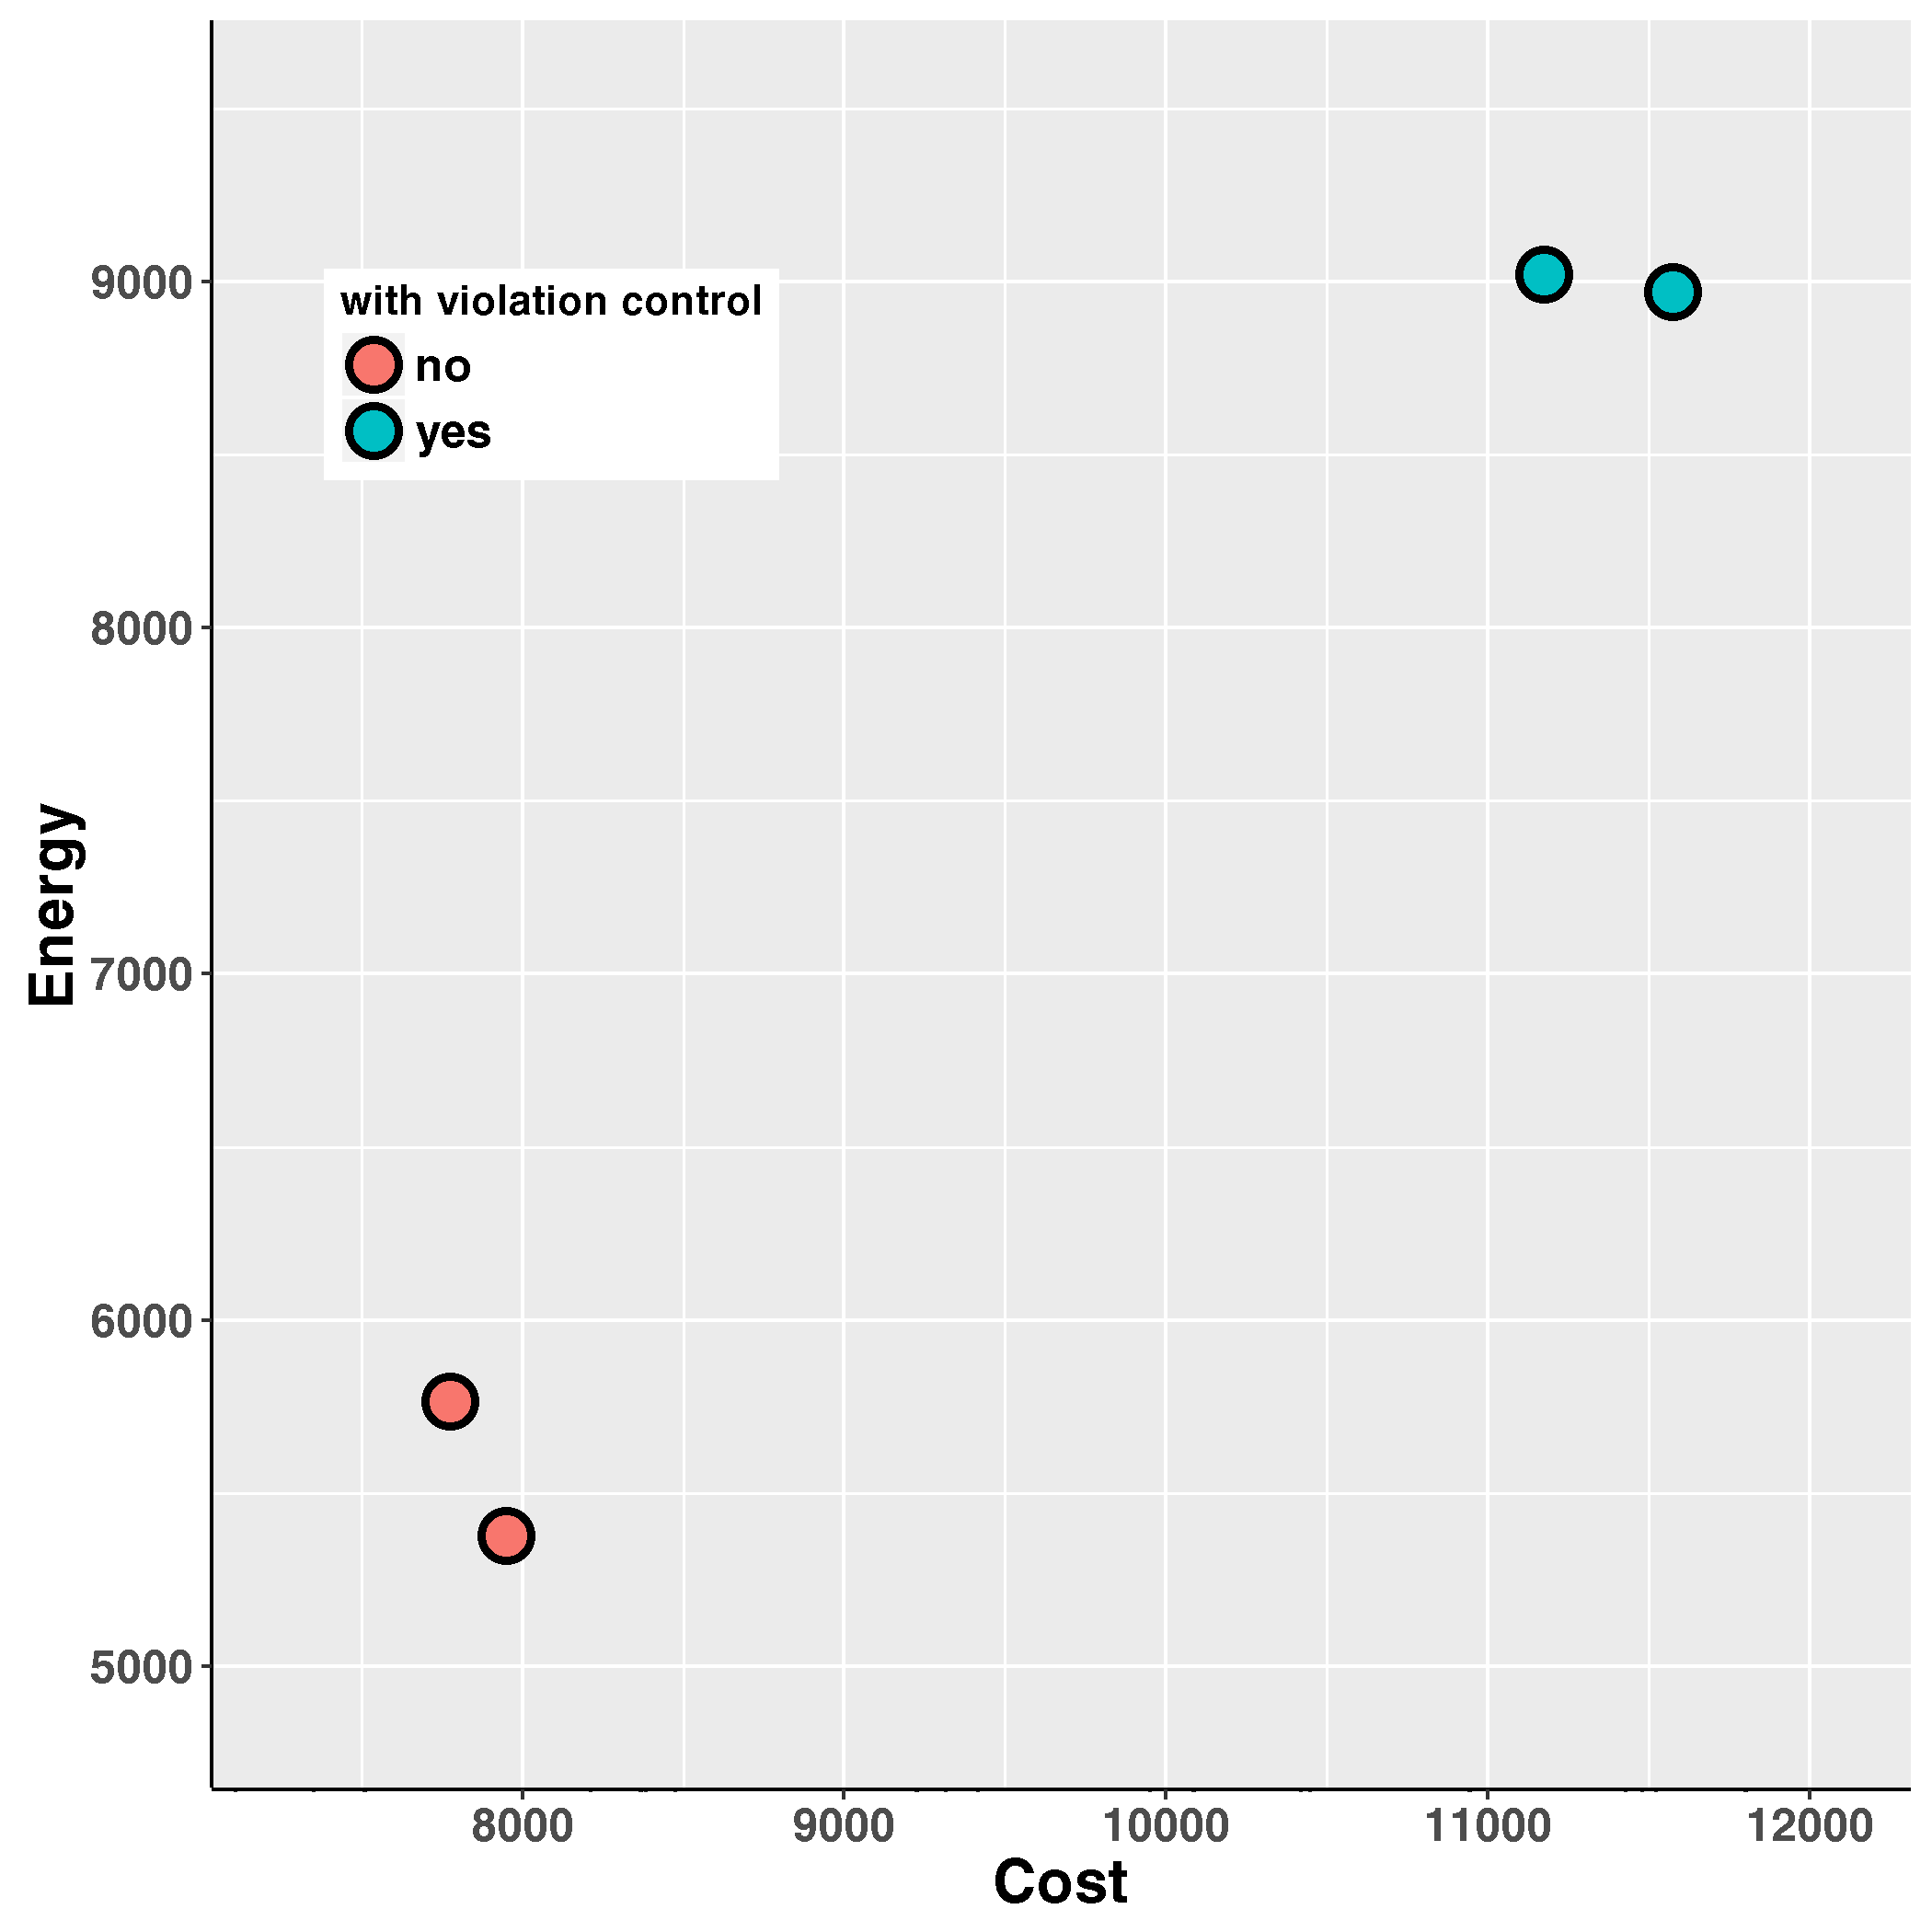
\includegraphics[width=\textwidth]{pics/preliminary/4/evolve.png}
   \caption{Problem 4}
   \label{fig:d}
   \end{subfigure}
   \begin{subfigure}[b]{0.45\textwidth}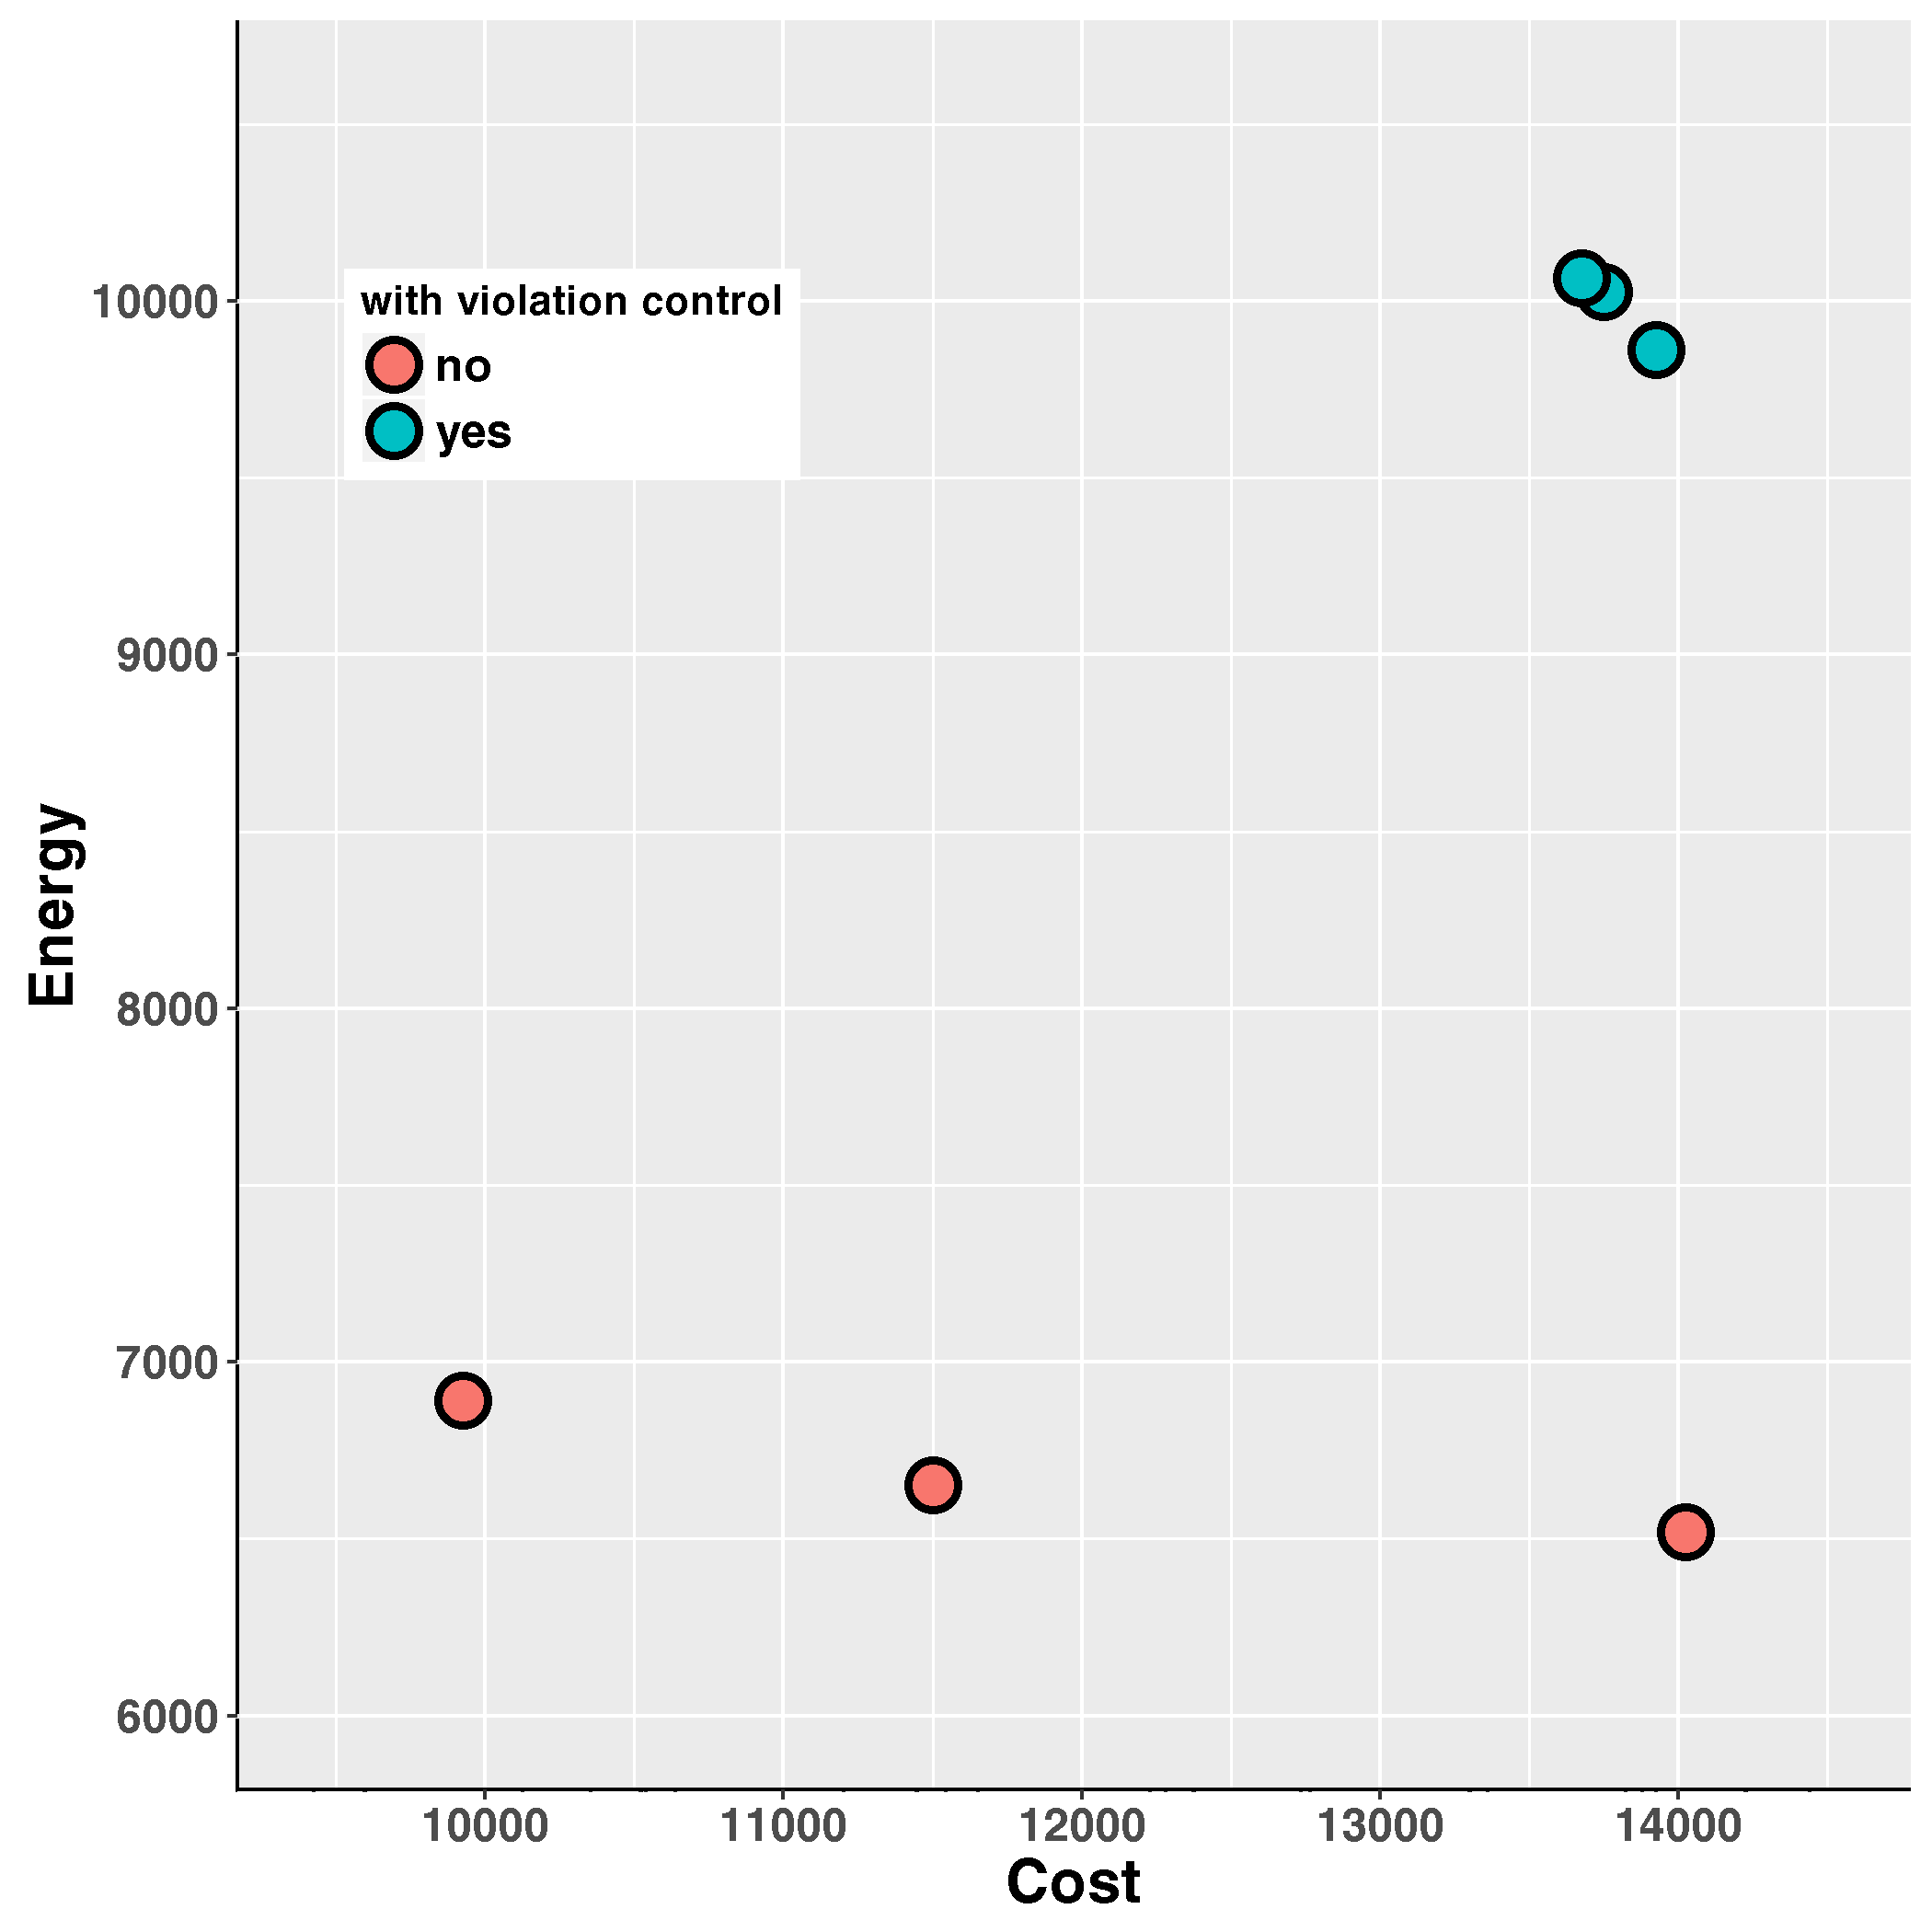
\includegraphics[width=\textwidth]{pics/preliminary/5/evolve.png}
   \caption{Problem 5}
   \label{fig:e}
   \end{subfigure}
     \begin{subfigure}[b]{0.45\textwidth}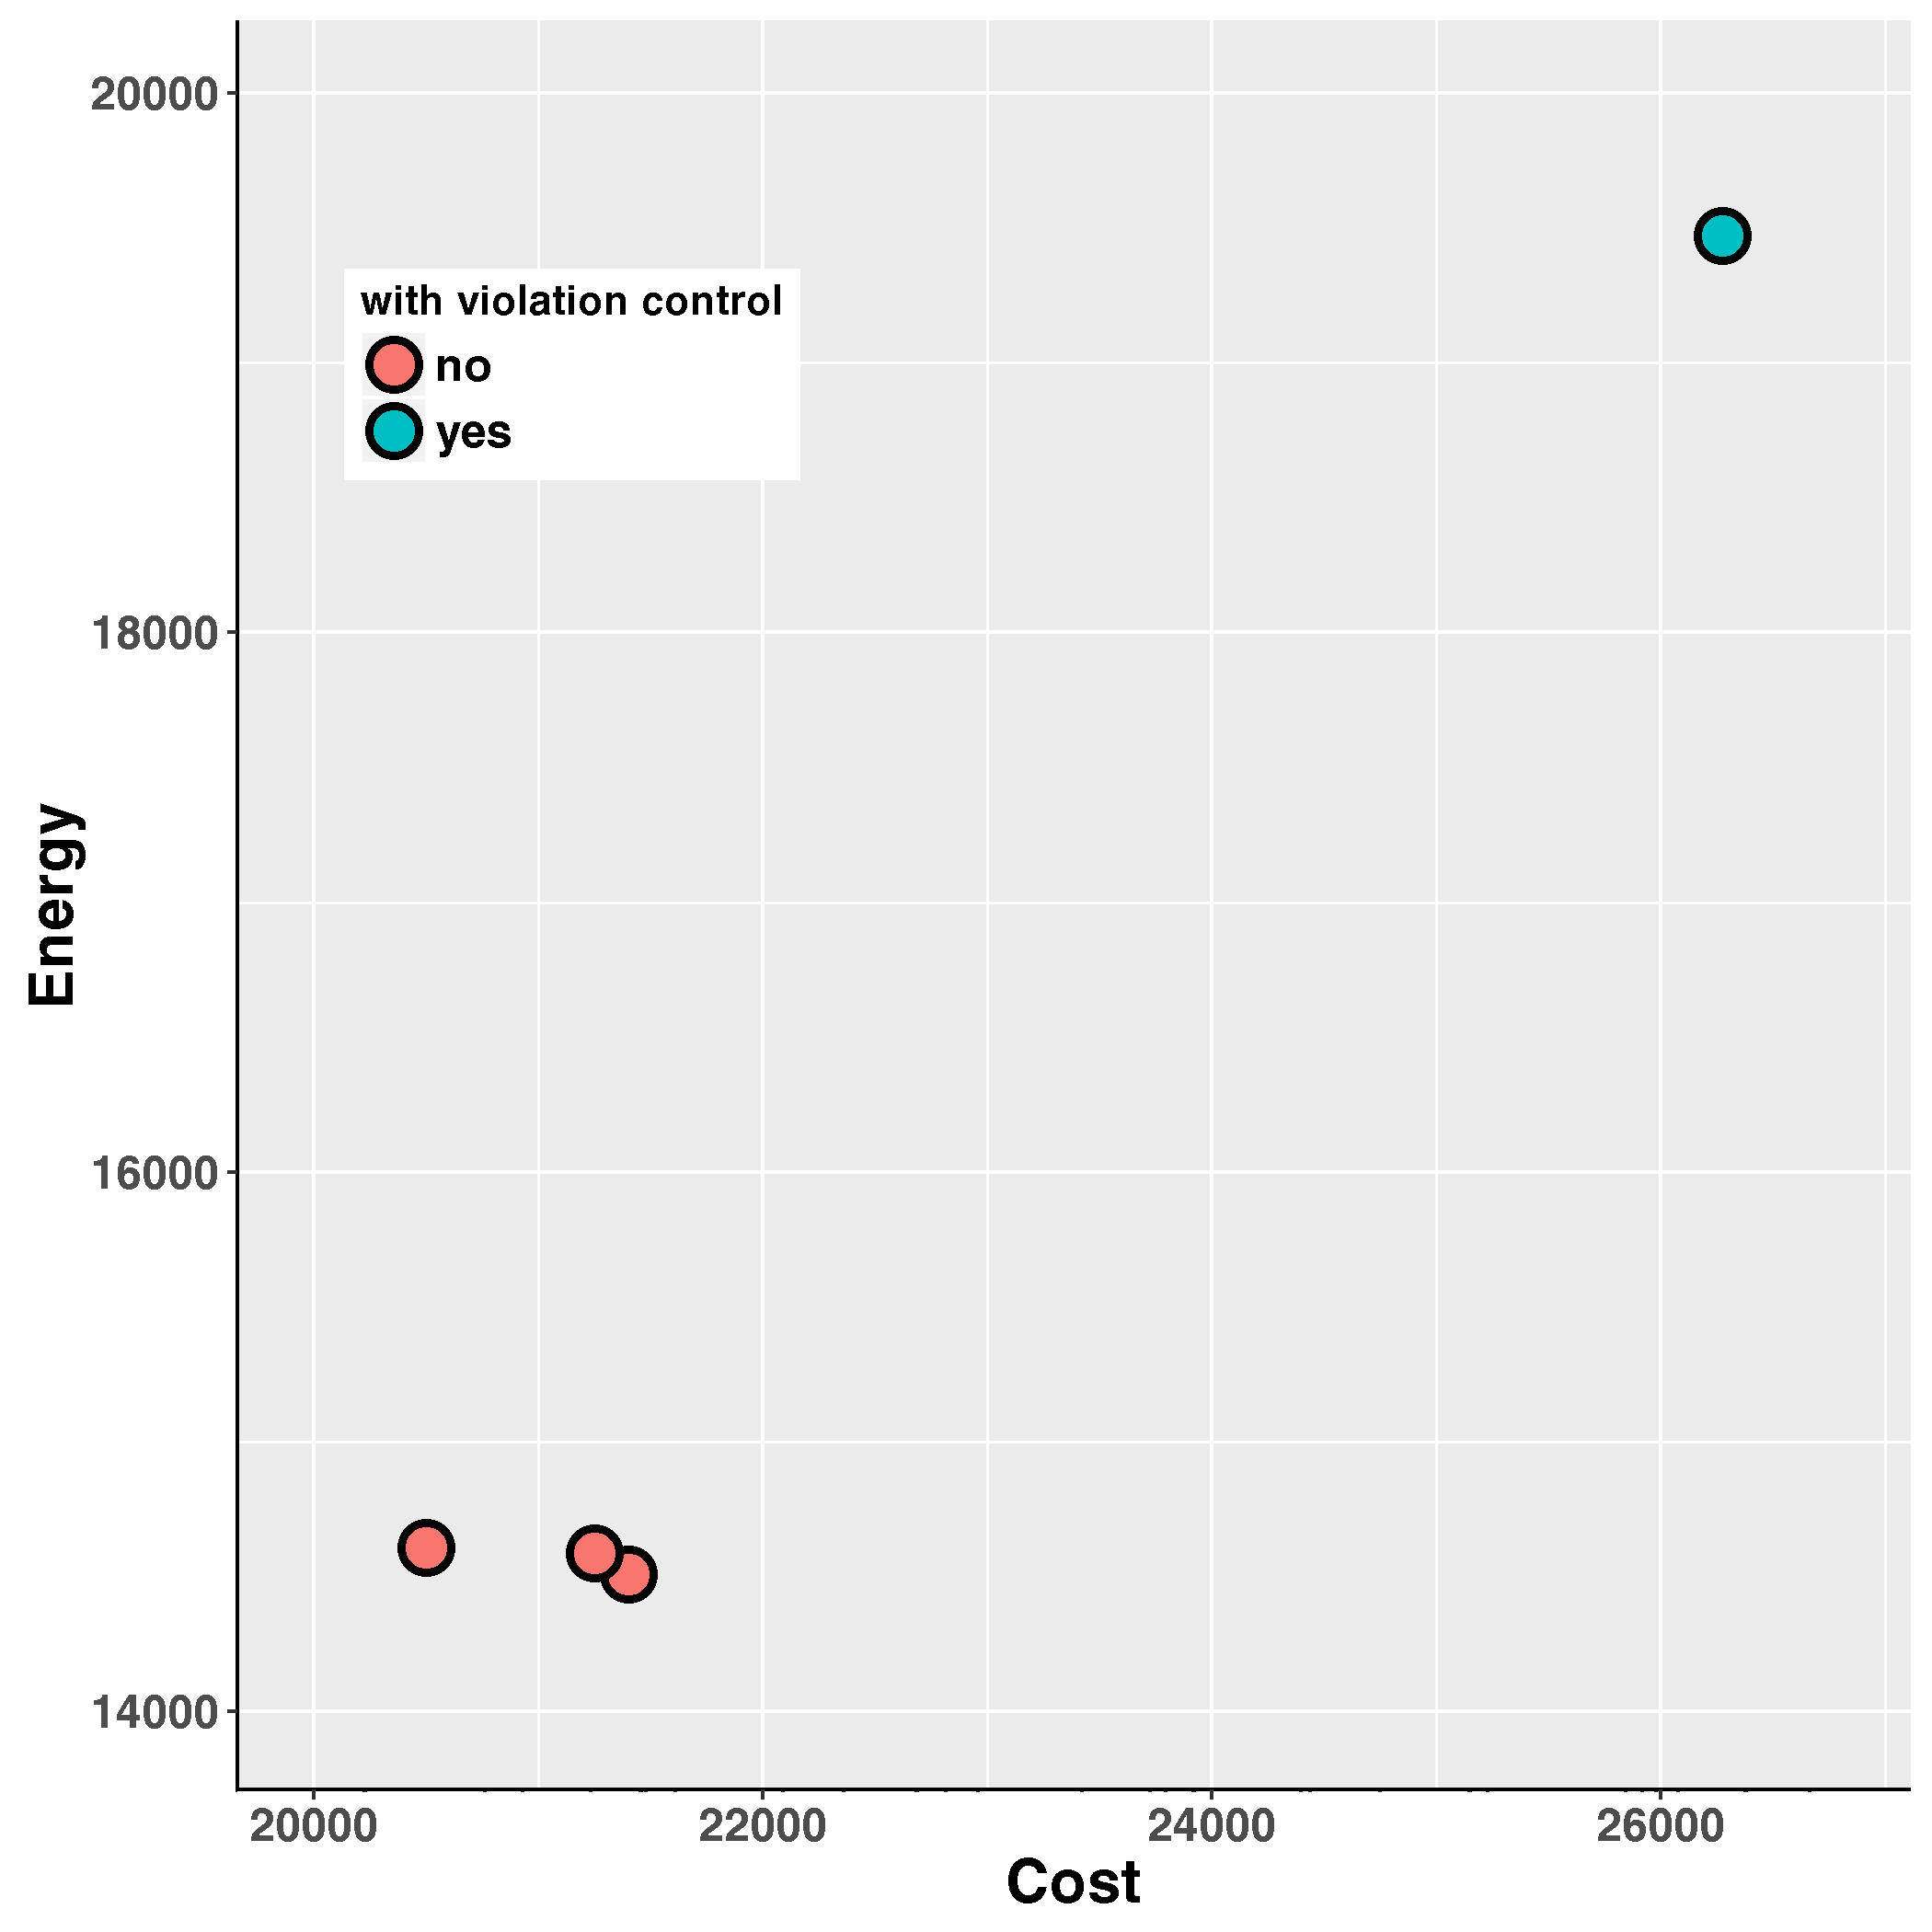
\includegraphics[width=\textwidth]{pics/preliminary/6/evolve.png}
   \caption{Problem 6}
   \label{fig:f}
   \end{subfigure}
   \caption{non-dominated solutions comparison between selection with violation control and without violation control}
   \label{fig:dynamicFunctions}
\end{figure}


\begin{table*}[!ht]
\centering
\caption{Comparison between two Mutation methods}
\label{tab:mutations}
\begin{tabular}{@{}cllll@{}}
\toprule
Problem & \multicolumn{2}{c}{roulette wheel mutation} & \multicolumn{2}{c}{Greedy mutation}   \\ \midrule
        & cost fitness         & energy fitness       & cost fitness      & energy fitness    \\
1       & 2664.6 $\pm$ 66.4      & 1652.42 $\pm$ 18.2     & 2661.7 $\pm$ 56.9   & 1653.2 $\pm$ 18.2   \\
2       & 6501.1 $\pm$ 130.2     & 4614.0 $\pm$ 110.7     & 6495.37 $\pm$ 110.7 & 4132.5 $\pm$ 80.4   \\
3       & 8939.2 $\pm$ 118.5     & 6140.7 $\pm$ 204.0     & 9020.5 $\pm$ 204.0  & 5739.6 $\pm$ 148.6  \\
4       & 11633.7 $\pm$ 301.1    & 9301.9 $\pm$ 254.0     & 12900.6 $\pm$ 243.0 & 9376.3 $\pm$ 120.9  \\
5       & 14102.0 $\pm$ 231.7    & 10164.8 $\pm$ 238.9    & 14789.2 $\pm$ 238.8 & 9876.3 $\pm$ 120.9  \\
6       & 27194.3 $\pm$ 243.0    & 19914.4 $\pm$ 307.5    & 27654.2 $\pm$ 307.5 & 19187.1 $\pm$ 176.6 \\ \bottomrule
\end{tabular}
\end{table*}

As we conducted the experiment for 30 runs, we first obtain an average non-dominated set over 30 runs by collecting the results from a specific generation from all 30 runs, and then apply a non-dominated sorting over them.

Firstly, we show the non-dominated solutions evolve along with the evolution process in Figure \ref{fig:evolve}.
These results come from selection method without violation control. 
As it illustrated, different colors represent different generations from 0th to 200th. 
For problem 1, because the problem size is small, the algorithm converged before 100 generations. Therefore, the non-dominated set from the 100th and 150th generations are overlapping with results from the 200th generation. For problem 2 and problem 3, it clearly shows the improvement of fitness values. For problem 4 onwards, the algorithm can only obtain a few solutions as the problem size is large, it is difficult to find solutions.

Then, the non-dominated sets of the last generation from two selection methods are compared in Figure \ref{fig:dynamicFunctions}. There are much fewer results are obtained from the violation control method throughout all cases. For the first three problems, the non-dominated set from the violation control method has similar quality
as the no violation control method. From problem 4 onwards, the results from selection with violation control are much worse in terms of fitness values. However, most of the results from non-violation control selection have a high violation rate. That is, the method without violation control is stuck in the infeasible regions and provide high-violation rate solutions. 

From figure \ref{fig:violations}, we can observe the violation rate between two methods.
It proves violation control has a great ability to prevent the individual from searching the infeasible region. On the other hand, without violation control, although, the algorithm can provide more solutions with better fitness values, most of them have a high violation rate over 10\% which are not very useful in reality.

As we mentioned in previous section, the mutation rate and consolidation factor are set differently for the two methods. For the method with violation control, the mutation rate is set to 0.9 and the consolidation factor $c$ is set to 0.01, this is because the feasible region is narrow and scattered. In order to avoid stucking in the local optima, a large mutation rate can help escape local optima. For the factor $c$, a larger percentage would easily lead the algorithm to infeasible regions. Therefore, it is set to a small number.





\begin{figure}
\centering
  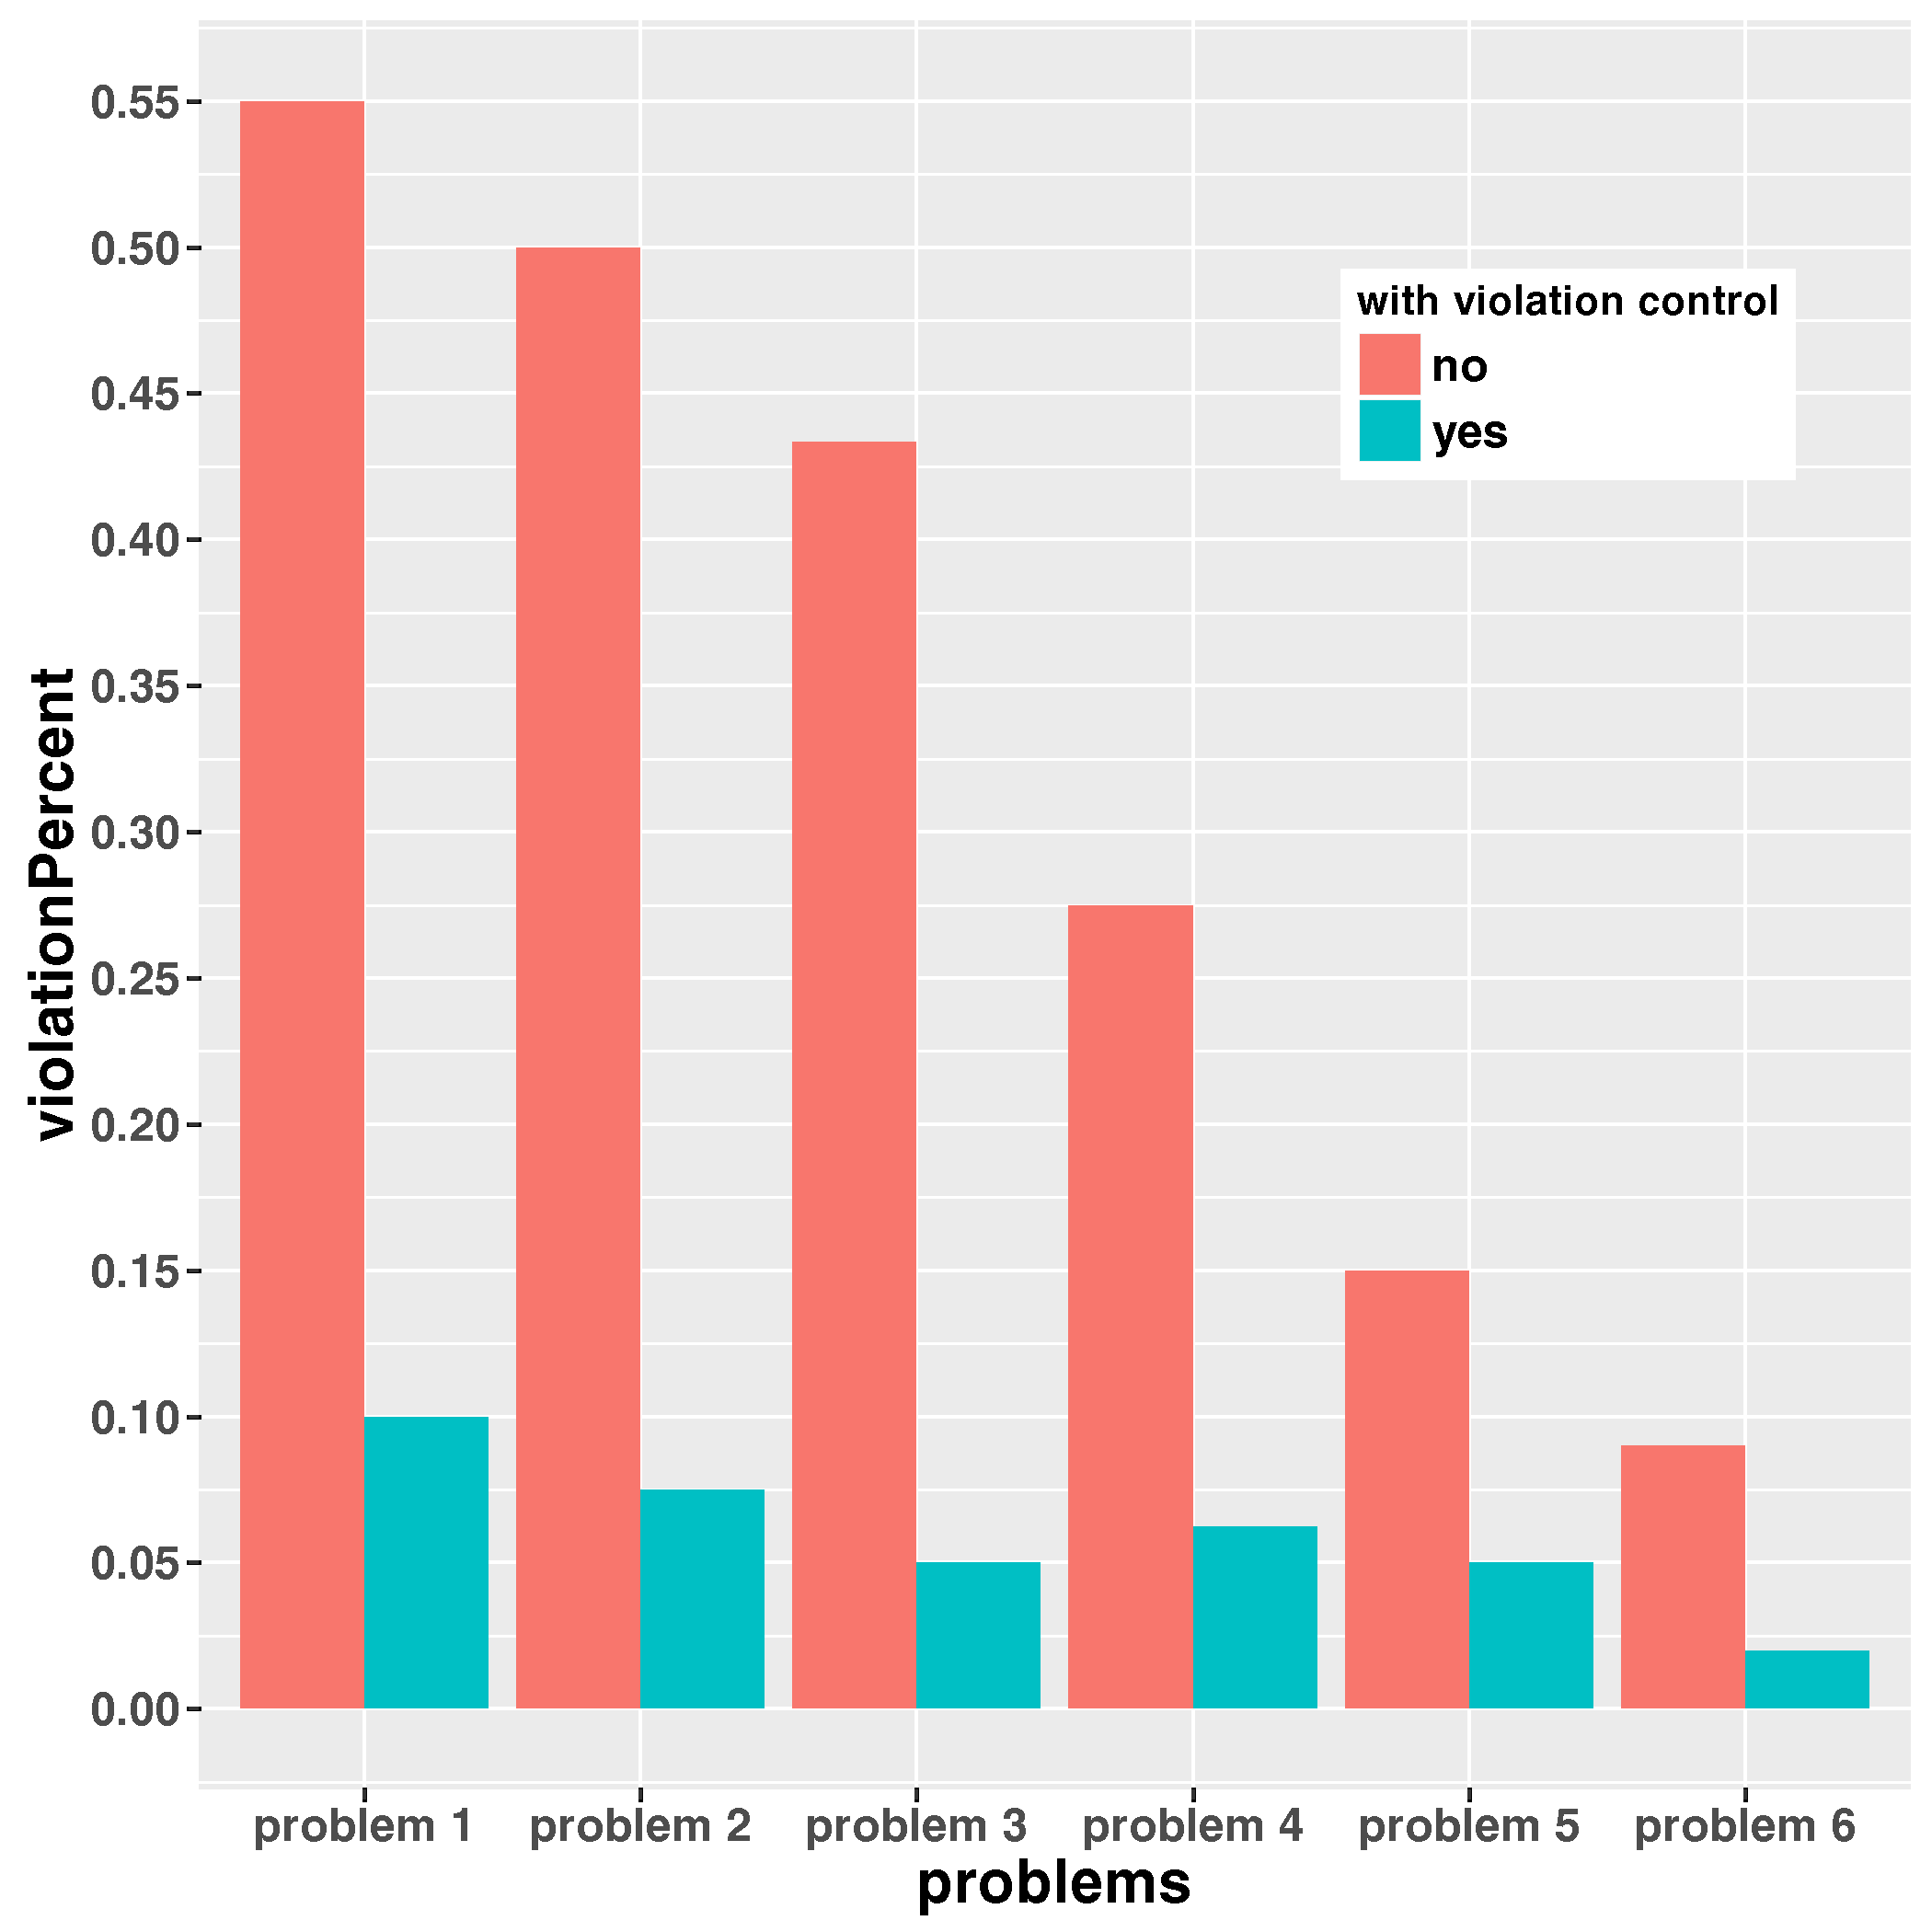
\includegraphics[width=.7\textwidth]{pics/preliminary/violations.png}
  \caption{Violation Percentage comparison between selection with violation control and without violation control}
  \label{fig:violations}
\end{figure}



\begin{flushleft}\textbf{Mutation with roulette wheel vs. Mutation with greedy algorithm}\end{flushleft}
Table \ref{tab:mutations} shows the fitness value comparison between mutation methods. According
to statistics significant test, there is little difference between methods. The possible reason
is the consolidation factor is set to 0.01. In each mutation iteration, there is only 1\% probability
that a service will be consolidated in an existed VM, therefore, the influence between
different consolidation strategies is trivial.





\section{Conclusion and Future work}
\label{sec:con}

This work investigates the bilevel model for the joint placement of container and VM. Several sub models such as workload model, power model were considered. A multi-objective formulation of the bilevel problem were established. Two objectives, minimizing the cost of used VMs and minimizing the energy consumption are achieved. In order to optimize the problem, we propose a NSGA-II based algorithm with specific designed representation which reduces the bilevel placement into one single-level. Genetic operators such as population initialization, mutation, selection were also designed for generating valid solutions and handling the constraints. The results are compared with different variances of the algorithm. The results show our approach can solve the very complicate optimization problem. With current work as a baseline, in future work, we could improve the quality of solutions as well as provide better violation control mechanisms.

